\chapter{Reduction of positive quadratic forms}\label{chap2}

\section{Quadratic forms}\label{chap2:sec1}\pageoriginale

Let $V$ be a vector space of dimension $n$ over the field $K$ of real
numbers. Define an inner product $\xi\eta$ between vectors $\xi$,
$\eta$ of $V$ by 
\begin{itemize}
\item[i)] $\xi\eta\in K$

\item[ii)] $\xi\eta=\eta\xi$

\item[iii)] $\xi(\eta+\zeta)=\xi\eta+\xi\zeta$

\item[iv)] $\xi(\eta a)=(\xi\eta)a$, $a\in K$.
\end{itemize}
Obviously if $\varepsilon_{1},\ldots,\varepsilon_{n}$ is a base of $V$ and
$\xi$, $\eta$ have the expression $\xi=\sum\limits_{i}$ $\varepsilon_i
a_{i}$, $\eta=\sum\limits_{i}\varepsilon_{i}b_{i}$ then
$$
\xi\eta=\sum^{n}_{i,j=1}a_{i}b_{j}(\varepsilon_{i}\cdot \varepsilon_{j}).
$$
If we denote by $S$ the $n$-rowed real matrix $S=(s_{ij})$,
$s_{ij}=\varepsilon_{i}\varepsilon_{j}$ then $S$ is symmetric and 
\begin{equation*}
\xi\eta=\ub{a}'S\ub{b}\tag{1}\label{c2:eq1}
\end{equation*}
where $\ub{a}=\left(\begin{smallmatrix} a_{1}\\ \vdots\\ a_{n}
\end{smallmatrix} \right)$, $\ub{b}=
\left(\begin{smallmatrix}b_{1}\\ \vdots\\ b_{n} 
\end{smallmatrix} \right)$ and $\ub{a}'$ denotes the transpose of the column
vector $\ub{a}$. \eqref{c2:eq1} is a bilinear form in the $2n$ quantities
$a_{1},\ldots,a_{n}$, $b_{1},\ldots,b_{n}$. In particular
$$
\xi^{2}=\ub{a}'S\ub{a}
$$
is a quadratic form in $a_{1},\ldots,a_{n}$.

Suppose\pageoriginale that $\varepsilon'_{1},\ldots,\varepsilon'_{n}$ is
another base of $V$. Then
$$
\varepsilon'_{i}=\sum_{j}\varepsilon_{j}a_{ij}\quad i=1,\ldots,n.
$$
and the matrix $A=(a_{ij})$ is non-singular. If
$S_{1}=(\varepsilon'_{i}\cdot\varepsilon'_{j})$ then one sees easily that
$$
S_{1}=S[A]=A'SA.
$$
Thus if $S$ with regard to one base is non-singular, then the $S$
corresponding to any other base is also non-singular.

Conversely let $S$ by and real $n$-rowed symmetric matrix and
$\varepsilon_{1},\ldots,\break\varepsilon_{n}$ a base of $V$ over $K$. Put 
$$
\varepsilon_{i}\cdot \varepsilon_{j}=s_{ij}\quad (j,i=1,\ldots,n)
$$
and extend it by linearity to any two vectors of $V$. Then we have in
$V$ an inner product defined.

If $\xi=\sum\limits_{i}\varepsilon_{i}x_{i}$ is a generic vector of $V$
over $K$,
$$
\xi^{2}=\ub{x}'S\ub{x}=S[x]=\sum_{i,j}x_{i}x_{j}s_{ij}.
$$
The expression on the right is a quadratic form in the $n$ variables
$x_{1},\ldots,\break x_{n}$ and we call $S$ its matrix. The quadratic form is
{\em degenerate} or {\em non-degenerate} according as its matrix $S$
is or is not singular.

Let $\ub{x}'S\ub{x}=\sum\limits^{n}_{k,l=1}s_{kl}x_{k}x_{l}$ be a
quadratic form in the $n$ variables $x_{1},\ldots,\break x_{n}$ and let
$s_{1}=s_{11}\neq 0$. We may write 
$$
\ub{x}'S\ub{x}=s_{1}x_{1}^{2}+2s_{12}x_{1}x_{2}+\cdots+2s_{1n}x_{1}x_{n}+Q(x_{2},\ldots,x_{n}) 
$$\pageoriginale
so that $Q(x_{2},\ldots,x_{n})$ is a quadratic form in the $n-1$
variables $x_{2},\ldots,x_{n}$. We now write, since $s_{1}\neq 0$,
\begin{gather*}
\ub{x}'S\ub{x} = s_{1}\left(x_{1}+\frac{s_{12}}{s_{1}} x_{2} +\cdots
+\frac{s_{1n}}{s_{1}} x_{n}\right)^{2} - \frac{s_{12}^{2}}{s_{1}}
x^{2}_{2}-\ldots\\  
-\frac{{s_{1n}}^2}{s_1} x^{2}_{n} + Q(x_{2},\ldots,x_{n}).
\end{gather*}
We have thus finally
$$
\ub{x}'S\ub{x}=s_{1}y^{2}_{1}+R(x_{2},\ldots,x_{n})
$$
where
$y_{1}=x_{1}+\dfrac{s_{12}}{s_{1}}x_{2}+\cdots+\dfrac{s_{1n}}{s_{1}}x_{n}$
and $R(x_{2},\ldots,x_{n})$ is a quadratic form in the $n-1$ variables
$x_{2},\ldots,x_{n}$. If we make a change of variables
\begin{equation*}
\left.
\begin{aligned}
y_{1} &=
x_{1}\frac{s_{12}}{s_{1}}x_{2}+\cdots+\frac{s_{1n}}{s_{1}}x_{n}\\
y_{1} &= x_{i}\hspace{2cm} i>1
\end{aligned}\right\}\tag{2}\label{c2:eq2}
\end{equation*}
then we may write
$$
\ub{x}'S\ub{x}=
\begin{pmatrix}
s_{1} & 0\\
0 & S_{1}
\end{pmatrix}
\begin{bmatrix}
y_{1}\\
\vdots\\
y_{n}
\end{bmatrix}
$$
where $S_{1}$ is the matrix of the quadratic form
$R(x_{2},\ldots,x_{n})$. Using matrix notation we have
\begin{equation*}
S=
\begin{pmatrix}
s_{1} & \ub{q}'\\
\ub{q} & S_{2}
\end{pmatrix}
=
\begin{pmatrix}
s_{1} & \ub{0}\\
\ub{0} & S_{1}
\end{pmatrix}
\begin{bmatrix}
1 & s^{-1}_{1}q'\\
\ub{0} & E
\end{bmatrix}
\tag{3}\label{c2:eq3}
\end{equation*}
where\pageoriginale $E$ is the unit matrix of order $n-1$, $\ub{q}$ is
a column of $n-1$ rows and
$$
S_{1}=S_{2}-s^{-1}_{1}\ub{q}\ub{q}';
$$
which, incidentally gives an expression for the matrix of $R$.

More generally suppose $S=\left(\begin{smallmatrix} S_{1} & Q\\ Q' &
  S_{2}\end{smallmatrix}\right)$ where $S_{1}$ is a $k$-rowed matrix
and is non-singular. Put $\ub{x}=\binom{\ub{y}}{\ub{z}}$ where
$\ub{y}$ is a column of $k$ rows and $\ub{z}$ has $n-k$ rows. Then
$$
S[\ub{x}]=S_{1}[y]+\ub{y}'Q\ub{z}+z'Q'\ub{y}+S_{2}[\ub{z}],
$$
which can be written in the form
\begin{equation*}
S[x]=S_{1}[\ub{y}+S^{-1}_{1}Q\ub{z}]+W[z]\tag{4}\label{c2:eq4}
\end{equation*}
where $W=S_{2}-Q'S^{-1}Q$. In matrix notation we have
\begin{equation*}
S=
\begin{pmatrix}
S_{1} & 0\\
0 & W
\end{pmatrix}
\begin{bmatrix}
E & S^{-1}_{1}Q\\
0 & E
\end{bmatrix}\tag{5}\label{c2:eq5}
\end{equation*}
the orders of the two unit matrices being evident. In particular, we
have
$$
|S|=|S_{1}|\;|W|.
$$

Let $S$ be a real, non-singular, $n$-rowed, symmetric matrix. It is
well known that there exists an orthogonal matrix $V$ such that 
$$
S[V]=V'SV=D
$$
where $D=[d_{1},\ldots,d_{n}]$ is a real diagonal matrix. The elements
$d_{1},\ldots,\break d_{n}$\pageoriginale of $D$ are called the eigen-values
of $S$. Let $\mathscr{L}$ denote the unit sphere
$$
\mathscr{L}:\ub{x'} \;\; \ub{x}=1 
$$
so that $a$ generic point $\ub{x}$ on $\mathscr{L}$ is an $n$-tuple
$\ub{x}=
\left(\begin{smallmatrix}x_{1}\\ \vdots\\ x_{n}\end{smallmatrix}
\right)$ of 
real numbers. Let $m$ and $N$ denote the smallest and largest of the
eigen values of $S$. Then for any $\ub{x}$ on $\mathscr{L}$.
$$
m\leq S[\ub{x}]\leq M
$$

For, if we put $\left(\begin{smallmatrix} y_{1}\\ \vdots\\ y_{n}
\end{smallmatrix}\right)=y-V^{-1}\ub{x}$, then $\ub{y}'\ub{y}=1$ and
$$
S[\ub{x}]=D[V^{-1}\ub{x}]=D[\ub{y}]=d_{1}y^{2}_{1}+\cdots+d_{n}y^{2}_{n}.
$$
But then
$$
S[\ub{x}]=(d_{1}-M)y^{2}_{1}+\cdots+(d_{n}-M)y^{2}_{n}+M \leq M.
$$
The other inequality is obtained by changing $S$ to $-S$.

More generally we have, for any arbitrary real vector $\ub{x}$
\begin{equation*}
m\ub{x}'\;\ub{x}\leq S[x]\leq M\ub{x}'\ub{x}.\tag{6}\label{c2:eq6}
\end{equation*}
If $\ub{x}=\ub{0}$, the statement is obvious. Let $\ub{x}\neq
\ub{0}$. Then $t^{2}=\ub{x}'\ub{x}\neq 0$. Put
$\ub{y}=t^{-1}\ub{x}$. Then $\ub{y}'y=1$ and so $m\leq S[\ub{y}]\leq
M$. Multiplying throughout by $t^{2}$ we get the result in \eqref{c2:eq6}.

We now define a quadratic form $\ub{x}'S\ub{x}$ to be {\em positive
  definite} (or simply positive) if $S[\ub{x}]>0$ for all vectors
$\ub{x}\neq \ub{0}$. It is {\em positive semi-definite} if
$S[\ub{x}]\geq 0$ for real $\ub{x}\neq 0$. We shall denote these by
$S>0$ and $S\geq 0$ respectively. If $S>0$, then\pageoriginale
obviously $|S|\neq 0$. For, if $|S|=0$, then there exists $\ub{x}\neq
0$ such that $S\ub{x}=\ub{0}$. Then
$$
0=\ub{x}'S\ub{x}>0
$$
which is absurd.

If $S>0$ and $|A|\neq 0$ and $A$ is a real matrix, then $T=S[A]$ is
again positive. For, if $\ub{x}=\ub{0}$, the $A\ub{x}\neq y\neq 0$ and
so
$$
T[\ub{x}]=S[A\ub{x}]=S[\ub{y}]>0.
$$

We now prove two lemmas for later use.

\begin{lem}\label{chap2:lem1}
A matrix $S$ is positive definite if and only if $|S_{r}|>0$ for
$r=1,\ldots,n$, where $S_{r}$ is the matrix formed by the first $r$
rows and columns of $S$.
\end{lem}

\begin{proof}
We shall use induction on $\ub{n}$. If $n=1$, the lemma is
trivial. Let therefore lemma be proved for matrices of order $n-1$
instead of $n$. Let
$$
S=
\begin{pmatrix}
S_{n-1} & \ub{q}\\
\ub{q}' & a
\end{pmatrix}
$$
If $S>0$ then $S_{n-1}>0$ and so $|S_{n-1}|\neq 0$. We can therefore
write
\begin{equation*}
S=
\begin{pmatrix}
S_{n-1} & \ub{0}'\\
\ub{0} & l
\end{pmatrix}
\begin{bmatrix}
E & S^{-1}_{n-1}\ub{q}\\
0 & l
\end{bmatrix}\tag{7}\label{c2:eq7}
\end{equation*}
so that $|S|=|S_{n-1}|l$. Induction hypothesis shows that
$|S_{n-1}|>0$ and $l>0$ so that $|S|>0$ and $|S_{r}|>0$ for all $r$. 
\end{proof}

The\pageoriginale converse also follows since by hypothesis $|S|>0$
and $|S_{n-1}|>0$. So $1>0$. But by induction hypothesis $S_{n-1}>0$.

\begin{lem}\label{chap2:lem2}
If $S>0$ and $S=(s_{kl})$, then
$$
|S|\leq s_{1}\ldots s_{n}
$$
where $s_{kk}=s_{k}$, $k=1,\ldots,n$.
\end{lem}

\begin{proof}
We again use induction on $\ub{n}$. From the equation \eqref{c2:eq7} we have
$$
|S|=|S_{n-1}|\cdot l.
$$
But $l=s_{n}-\ub{q}'S^{-1}_{n-1}\ub{q}>0$ since $S^{-1}_{n-1}>0$ and
$s_{n}>0$. If we assume lemma proved for $n-1$ instead of $n$ we get
$$
|S|\leq s_{1}\ldots s_{n-1} l \leq s_{1}\ldots s_{n}.
$$

More generally we can prove that if $S>0$ and
$S=\left(\begin{smallmatrix} S_{1} & S_{12}\\ S'_{12} & S_{2}
\end{smallmatrix}\right)$ then
\begin{equation*}
|S|\leq |S_{1}|\cdot |S_{2}|\tag{8}\label{c2:eq8}
\end{equation*}
It is easy to see that equality holds in \eqref{c2:eq8} if and only if
$S_{12}=0$.

Let $S>0$, then $s_{1},\ldots,s_{n}$ are all positive. We can write as
in \eqref{c2:eq3}
$$
S=
\begin{pmatrix}
s_{1} & \ub{0}\\
\ub{0} & W
\end{pmatrix}
\begin{bmatrix}
1 & s^{-1}_{1}\ub{q}'\\
\ub{0} & E
\end{bmatrix}
$$
But\pageoriginale since now $W>0$, its first diagonal element is
different from zero and we can write $W$ also in the form \eqref{c2:eq3}. In this
way we get
\begin{equation*}
S=
\begin{pmatrix}
d_{1} &  & 0\\
 &\ddots &\\
0 & & d_{n}
\end{pmatrix}
\begin{bmatrix}
1, & d_{12},\ldots,d_{1n}\\
0, & 1,d_{23},\ldots,d_{2n}\\
: &\ldots\ldots\\
0 &\ldots\ldots 1
\end{bmatrix}
=D[V]\tag{9}\label{c2:eq9}
\end{equation*}
where $D=[d_{1},\ldots,d_{n}]$ is a diagonal matrix and $V=(d_{kl})$
is a triangle matrix with $d_{kk}=1$, $k=1,\ldots,n$, and $d_{kl}=0$,
$k>1$. We can therefore write
$$
S[\ub{x}]=\sum^{n}_{k=1}d_{k}(x_{k}+d_{k\;k+1}x_{k+1}+\cdots+d_{kn}x_{n})^{2}
$$

The expression $S=D[V]$ is {\em unique}. For if $S=D_{1}[V_{1}]$ where
$D_{1}$ is a diagonal matrix and $V_{1}$ is triangular, then
$$
D[W]=D_{1}
$$
where $W=VV^{-1}_{1}$ is also a triangular matrix. In this case, it
readily follows that $W=E$ and $D=D_{1}$.

In general we have the fact that if
\begin{equation*}
S=
\begin{pmatrix}
S & 0\\
0 & S_{2}
\end{pmatrix}
\begin{bmatrix}
E & T\\
0 & E
\end{bmatrix}\tag{10}\label{c2:eq10}
\end{equation*}
where $S_{1}$ has order $k$ then $S_{1}$, $S_{2}$ and $T$ are unique.

We call the decomposition \eqref{c2:eq9} of $S$ the {\em Jacobi transformation}
of $S$. 
\end{proof}

\section{Minima of definite forms}\label{chap2:sec2}\pageoriginale

Let $S$ and $T$ be two real, non-singular $n$-rowed symmetric
matrices. They are said to be {\em equivalent} (denoted $S\sim T$) if
there exists a unimodular matrix $U$ such that
$$
S[U]=T.
$$
Since the unimodular matrices form a group, the above relation is an
equivalence relation. We can therefore put the $n$-rowed real
symmetric matrices into {\em classes} of equivalent
matrices. Evidently, two matrices in a class have the same
determinant.

If $S=S'$ is real and $t$ is a real number, we say that $S$ {\em
  represents $t$ integrally}, if there is an integral vector $\ub{x}$
such that
$$
S[\ub{x}]=t.
$$
In case $t=0$, we insist that $\ub{x}\neq \ub{0}$. The representation
is said to be {\em primitive}, if $\ub{x}$ is a primitive
vector. Obviously if $S\sim T$ then $S$ and $T$ both represent the
same set of real numbers.

If $S>0$, then all the eigen values of $S$ are positive. Let $m>0$ be
the smallest eigen value of $S$. Let $t>0$ be a large real
number. Then if $S[\ub{x}]<t$ then $m\ub{x}'\ub{x}<t$ and so the
elements of $\ub{x}$ are bounded. Therefore there exist only finitely
many integral vectors $\ub{x}$ satisfying
$$
S[\ub{x}]<t.
$$
This means that if $\ub{x}$ runs through all non-zero integral
vectors, $S[\ub{x}]$ has a minimum. We denote this minimum by
$\mu(S)$. There is therefore\pageoriginale an integral $\ub{x}$ such that
$$
S[\ub{x}]=\mu(S).,\quad \ub{x}\neq \ub{0}. 
$$
Moreover $\ub{x}$ is a primitive vector. For if $\ub{x}$ is not
primitive, then $\ub{x}=q\ub{y}$ where $q>1$ is an integer, and
$\ub{y}$ is a primitive vector. Then 
$$
\mu(S)=S[\ub{x}]=q^{2}S[\ub{y}]>S[\ub{y}]
$$
which is impossible. Furthermore if $S\sim T$ then
$\mu(S)=\mu(T)$. For, let $S=T[U]$ where $U$ is unimodular. If
$\ub{x}$ is a primitive vector such that $\mu(S)=S[\ub{x}]$, then 
$$
\mu(S)=S[\ub{x}]=T[U\ub{x}]\geq \mu(T).
$$
Also if $\mu(T)=T[\ub{y}]$, then
$$
\mu(T)=T[\ub{y}]=S[U^{-1}\ub{y}]\geq \mu(S).
$$
This proves the contention.

If $S>0$ and $t$ is a real number, then $\mu(tS)=t\mu(S)$. But
$|tS|=t^{n}|S|$ so that it seems reasonable to compare $\mu(S)$ with
$|S|^{1/n}$.

We not prove the following important theorem due to {\em Hermite}.

\setcounter{thm}{0}
\begin{thm}\label{chap2:thm1}
If $\mu(S)$ is the minimum of the positive matrix $S$ of $n$ rows,
there exist a constant $c_{n}$ depending only on $n$, such that
$$
\mu(S)\leq c_{n}|S|^{1/n}
$$
\end{thm}

\begin{proof}
We use induction on $n$.
\end{proof}

If\pageoriginale $n=1$, then $S$ is a positive real number $s$. If
$x\neq 0$, and integral, then $sx^{2}>s$ unless $x=\pm 1$ so that
$$
c_{1}=1.
$$
Let us assume theorem proved for $n-1$ instead of $n$. Let $\ub{x}$ be
the primitive integral vector such that $\mu(S)=S[\ub{x}]$. Complete
$\ub{x}$ into a unimodular matrix $U$. Then $T=S[U]$ has first
diagonal element equal to $\mu(S)$. Also $\mu(S)=\mu(T)$ by our
remarks above. Furthermore $|S|=|T|$. Therefore in order to prove the
theorem we may assume that the first diagonal element $s_{1}$ of $S$
is equal to $\mu(S)$.
\begin{align*}
\text{Let \quad} S&= 
\begin{pmatrix}
s_{1} & \ub{q}'\\
\ub{q} & S_{1}
\end{pmatrix}
.\text{ Then}\\
S&= 
\begin{pmatrix}
s_{1} & \ub{0}'\\
\ub{0} & W
\end{pmatrix}
\begin{bmatrix}
1 & s^{-1}_{1}\ub{q}'\\
\ub{0} & E
\end{bmatrix}
\end{align*}
where $W=S_{1}-\ub{q}s^{-1}_{1}\ub{q}$! Also $|S|=s_{1}|W|$.

Let $\ub{x}=\binom{x_{1}}{\ub{y}}$ be a vector and let $\ub{y}$ have
$n-1$ rows, so that
\begin{equation*}
S[\ub{x}]=s_{1}(x_{1}+s^{-1}_{1}\ub{q}'\ub{y})^{2}+W[y].\tag{11}\label{c2:eq11}
\end{equation*}
Since $W>0$, we can choose an integral $\ub{y}$ so that $W[\ub{y}]$ is
minimum. $x_{1}$ can now be chosen integral in such a manner that
\begin{equation*}
- \frac{1}{2}\leq x_{1}+s^{-1}_{1}\ub{q}'\ub{y}\leq \frac{1}{2}\tag{12}\label{c2:eq12}
\end{equation*}
using\pageoriginale \eqref{c2:eq11} and \eqref{c2:eq12} and induction hypothesis we get
$$
\mu(S)\leq S[\ub{x}]\leq \frac{\mu(S)}{4}+c_{n-1}\big | W \big|^{1/(n-1)}
$$
Substituting for $|W|$ we get
$$
\mu(S)\leq
\left(\frac{4}{3}c_{n-1}\right)^{\frac{n-1}{n}}|S|^{\frac{1}{n}}
$$
which proves the theorem.

Using $c_{1}=1$ and computing successively from the recurrence formula
$c_{n}=\left(\dfrac{4}{3}c_{n-1}\right)^{\frac{n-1}{n}}$ we see that
\begin{equation*}
c_{n}=(4/3)^{\frac{n-1}{2}}\tag{13}\label{c2:eq13}
\end{equation*}
is a possible value of $c_{n}$. This estimate is due to {\em Hermite}.

The best possible value for $c_{n}$ is unknown except in a few
cases. We shall show that $c_{2}=\sqrt{\dfrac{4}{3}}$ and that it is
the best possible for $n=2$. From Hermite's estimate \eqref{c2:eq13}, we
see that for a positive binary matrix $S$,
$$
\mu(S)\leq \left(\frac{4}{3}\right)^{\frac{1}{2}}|S|^{\frac{1}{2}}.
$$
Consider now the positive quadratic from $x^{2}+xy+y^{2}$ whose matrix
$$
S=
\begin{pmatrix}
1 & \frac{1}{2}\\
\frac{1}{2} & 1
\end{pmatrix}
$$
For integral $x$, $y$ not both zero, $x^{2}+xy+y^{2}\geq 1$ so that
$\mu(S)=1$. Also $|S|=\dfrac{3}{4}$. We have
$$
1=\left(\frac{4}{3}\right)^{\frac{1}{2}}|S|^{\frac{1}{2}}
$$
which\pageoriginale proves that $\sqrt{\dfrac{4}{3}}$ is the best
possible value of $c_{2}$.

We shall now obtain a `finer' estimate for $c_{n}$ due to {\em
  Minkowski}. This estimate is better than Hermite's for {\em large}
values of $n$. To this end we make the following consideration.

Let $R_{n}$ denote the Euclidean space of $n$ dimensions regarded as a
vector space of ordered $n$-tuples $(x_{1},\ldots,x_{n})$. A point set
$\mathscr{L}$ in $R_{n}$ is said to be {\em convex} if whenever $A$
and $B$ are two points of it, $\dfrac{A+B}{2}$, the mid point of the
line joining $A$ and $B$, is also a point of $\mathscr{L}$. It is said
to be {\em symmetric} about the origin if whenever $x$ belongs to it,
$-x$ also belongs to it. Obviously if $\mathscr{L}$ is both convex and
symmetric, it contains the origin.

If $\mathscr{L}$ is a point set in $R_{n}$ and $h$ is any point in
$R_{n}$ we denote by $\mathscr{L}_{h}$ the set of points $x$ such that
$x\in\mathscr{L}_{h}$ if and only if $x-h$ is a point of
$\mathscr{L}$. With this notation $\mathscr{L}=\mathscr{L}_{0}$.

If $\mathscr{L}$ is an open, bounded symmetric convex set, the
$\mathscr{L}$ has a measure $\nu(\mathscr{L})$ in the Jordon sense and
for $h\in R_{n}$
$$
\nu(\mathscr{L})=\nu(\mathscr{L}_{h}).
$$

We call a point $P=(x_{1},\ldots,x_{n})$ in $R_{n}$ a {\em lattice
  point} if $x_{1},\ldots,x_{n}$ are all integers. The lattice points
form a lattice in $R_{n}$ considered as a vector group. We shall
denote points of this lattice by the letters $g$, $g',\ldots$.

The following lemma, due to {\em Minkowski}, shows the relationship
between convex sets and lattices.

\begin{lem}\label{chap2:lem3}
If\pageoriginale $\mathscr{L}$ is an open, bounded, symmetric and
convex set of volume $>2^{n}$, then $\mathscr{L}$ contains a lattice
point other than the origin.
\end{lem}

\begin{proof}
We shall assume that $\mathscr{L}$ has no lattice point in it other
than the origin and then prove that $\nu(\mathscr{L})\leq 2^{n}$.
\end{proof}

So let $\mathscr{L}$ have no lattice point in it other than the
origin. Define the point set $\mathscr{M}$ by $x\in\mathscr{M}$ if and
only if $2x\in\mathscr{L}$. Then $\mathscr{M}$ is an open, symmetric,
bounded and convex set. Also
\begin{equation*}
\nu(\mathscr{L})=2^{n}\nu(\mathscr{M}).\tag{14}\label{c2:eq14}
\end{equation*}

Consider now the translates $\mathscr{M}_{g}$ of $\mathscr{M}$ by the
lattice points. If $g\neq g'$ then $\mathscr{M}_{g}$ and
$\mathscr{M}_{g'}$ are disjoint sets. For, if $x\in\mathscr{M}_{g}\cap
\mathscr{M}_{g'}$ then $x-g$ and $x-g'$ are points of
$\mathscr{M}$. Since $\mathscr{M}$ is symmetric and convex.
$$
\frac{g-g'}{2}=\frac{(x-g')+(g-x)}{2}
$$
is a point of $\mathscr{M}$. By definition of $\mathscr{M}$, $g - g'$ is
a point of $\mathscr{L}$. But $g\neq g'$. Thus $\mathscr{L}$ has a
lattice point other than the origin. This contradicts our
assumption. Thus the $\mathscr{M}_{g}$ for all $g$ are distinct.

Let $\varepsilon$ denote the unit cube, that is the set of points
$x=(x_{1},\ldots,x_{n})$ with $0\leq x_{i}<1$, $i=1,\ldots,n$. By the
property of $\mathscr{M}_{g}$'s above
\begin{equation*}
\sum_{g}\nu(\mathscr{M}_{g}\cap \varepsilon)=\nu(\varepsilon\cap
\sum_{g}\mathscr{M}_{g})\leq \nu(\varepsilon)=1\tag{15}\label{c2:eq15}
\end{equation*}
But $\nu(\mathscr{M}_{g}\cap
\varepsilon)=\nu(\mathscr{M}\cap\varepsilon_{-g})$ so that by \eqref{c2:eq15}
$$
1\geq
\sum_{g}\nu(\varepsilon\cap\mathscr{M}_{g})=\sum_{g}\nu(\varepsilon_{-g}\cap\mathscr{M})=\nu(\sum_{g}\varepsilon_{-g}\cap\mathscr{M}). 
$$
But\pageoriginale the $\varepsilon_{-g}$ cover $R_{n}$ completely without gaps or
overlapping when $g$ runs over all lattice points. Hence
$$
\nu(\mathscr{M})\leq 1.
$$
Using \eqref{c2:eq14} our theorem follows.

We can now prove the following theorem due to {\em Minkowski}.

\begin{thm}\label{chap2:thm2}
If $S>0$ and $\mu(S)$ is its minimum, then 
$$
\mu(S)\leq \frac{4}{\pi}\cdot
\left\{\Gamma\left(\frac{n}{2}+1\right)\right\}^{2/n}|S|^{1/n} 
$$
\end{thm}

\begin{proof}
In $R_{n}$ let us consider the point set $\mathscr{L}$ defined by the
set of $\ub{x}=\left(\begin{smallmatrix}
  x_{1}\\ \vdots\\ x_{n}\end{smallmatrix}\right)$ with
$$
S[\ub{x}]< \rho
$$
It is trivially seen to be open and symmetric. Also since $S>0$,
$\mathscr{L}$ is bounded. To see that it is convex, write $S=A'A$ and
put $A\ub{x}_{1}=\ub{y}_{1}$, $A\ub{x}_{2}=\ub{y}_{2}$. Then a simple
calculation proves that
$$
2\left(\frac{y_{1}+y_{2}}{2}\right)'\left(\frac{\ub{y}_{1}+\ub{y}_{2}}{2}\right)\leq 
\ub{y}'_{1}\ub{y}_{1}+\ub{y}'_{2}\ub{y}_{2}. 
$$ 
This shows that $\mathscr{L}$ is a convex set. The volume of
$\mathscr{L}$ is
$$
\nu(\mathscr{L}) = \frac{\rho^{n/2} \pi^{n/2}}{\Gamma(\frac{n}{2}+1)}
\big| S \big|^{- \,1/2}
$$
If\pageoriginale we put $\rho=\mu(S)$, then $\mathscr{L}$
contains no lattice point other than the origin. Minkowski's lemma
then proves theorem \ref{chap2:thm2}.
\end{proof}

Denote the constants in Hermite's and Minkowski's theorems by $c_{n}$
and $c'_{n}$ respectively. If we use stirling's formula for the
$\Gamma$-function in the form
$$
\log\Gamma(x)\sim x\log x.
$$
We get $\log
c'_{n} = \log\dfrac{4}{\pi} + \dfrac{2}{n} \log \Gamma
\left(\dfrac{n}{2}+1\right)\sim\log 
n$ whereas $\log c_{n}=\dfrac{n-1}{2}\log 4/3\sim\lambda n$ where
$\lambda$ is an absolute constant. This shows that for large $n$,
Minkowski's estimate is better than Hermite's. 

\section{Half reduced positive forms}\label{chap2:sec3}

We now consider the space $R_{h}$, $h=\dfrac{n(n+1)}{2}$ of real
symmetric $n$-rowed matrices and impose on it the topology of the
$h$-dimensional real Euclidean space. Let $\mathscr{P}$ denote the
subspace of positive matrices. If $S\in\mathscr{P}$ then all the
principal minors of $S$ have positive determinant. This shows that
$\mathscr{P}$ is the intersection of a finite number of open subsets
of $R_{h}$ and hence is open.

Let $S$ be a matrix in the frontier of $\mathscr{P}$ in $R_{h}$. Let
$S_{1}, S_{2},\ldots$ be a sequence of matrices in $\mathscr{P}$
converging to $S$. Let $\ub{x}\neq \ub{0}$ be {\em any} real column
vector. Then $S_{k}[\ub{x}]>0$ and hence by continuity $S[\ub{x}]\geq
0$. From the arbitrariness of $\ub{x}$, it follows that $S\geq 0$. On
the other hand let $S$ be any positive semi-definite matrix in
$R_{h}$. Let $E$ denote the unit matrix of order $n$. Then for
$\varepsilon>0$, $S+\varepsilon E$ is a positive matrix, which shows that
in\pageoriginale every neighbourhood of $S$ there are points of
$\mathscr{P}$. This proves that the frontier of $\mathscr{P}$ in
$R_{h}$ consists precisely of positive semi-definite matrices.

Let $\Gamma$ denote the group of unimodular matrices. We represent
$\Gamma$ in $R_{h}$ as a group of transformations $S\to S[U]$, $S\in
R_{h}$. Also $U$ and $-U$ load to the same representation in
$R_{h}$. It is easy to see that the only elements in $\Gamma$ which
keep every element of $R_{h}$ fixed are $\pm E$. Thus if we identify
in $\Gamma$, the matrices $U$ and $-U$ then $S\to S[U]$ gives a
faithful representation of $\Gamma_{0}$ in $R_{h}$,
$\Gamma_{0}=\Gamma/\pm E$. If $U$ runs over all elements of $\Gamma$
and $S\in R_{h}$, $S[U]$ runs through all matrices in the class of
$S$. We shall now find in each class of positive matrices, a matrix
having certain `nice' properties.

Let $T\in\mathscr{P}$ and let $\ub{u}$ run over the first columns of
all the matrices in $\Gamma$. There $\ub{u}$ are precisely all the
primitive vectors. Consider the values $T[\ub{u}]$ as $\ub{u}$ runs
over these first columns. Then $T[\ub{u}]$ has a minimum, which is
none other than $\mu(T)$. Let this be attained for
$\ub{u}=\ub{u}_{1}$. It is obvious that $\ub{u}_{1}$ is not unique
for, $-\ub{u}_{1}$, also satisfies this condition. In any case, since
$T>0$, there are only finitely many $\ub{u}$'s with the property
$T[\ub{u}]=T[\ub{u}_{1}]$. Let $\ub{u}_{1}$ be fixed and let $\ub{u}$
run over the second columns of all unimodular matrices whose first
column is $\ub{u}_{1}$. The $\ub{u}$'s now are {\em not} all the
primitive vectors (for instance $\ub{u}\neq \ub{u}_{1}$). $T[\ub{u}]$
again has a minimum say for $\ub{u}=\ub{u}_{2}$ and by
our\pageoriginale remark above
$$
T[\ub{u}_{1}]\leq T[\ub{u}_{2}]
$$
Also there are only finitely many $\ub{u}$ with
$T[\ub{u}]=T[\ub{u}_{2}]$. Consider now all unimodular matrices whose
first two columns are $\ub{u}_{1}$, $\ub{u}_{2}$ and determine a
$\ub{u}_{3}$ such that $T[\ub{u}_{3}]$ is minimum. Continuing in this
way one finally obtains a unimodular matrix
$$
U=(\ub{u}_{1},\ldots,\ub{u}_{n})
$$
and a positive matrix $S=T[U]$.

$S\sim T$ and by our construction, it is obvious, that $S$ is not
unique in the class of $T$. We shall study the matrices $S$ and $U$
more closely.

Suppose we have constructed the columns
$\ub{u}_{1},\ldots,\ub{u}_{k-1}$. In order to construct the $k$-th
column we consider all unimodular matrices $V$ whose first $k-1$
columns are $\ub{u}_{1},\ldots,\ub{u}_{k-1}$ in that order. Using the
matrix $U$ above which has this property, 
\begin{equation*}
U^{-1}V=
\begin{pmatrix}
E_{k-1} & A\\
0 & B
\end{pmatrix}
\tag{16}\label{c2:eq16}
\end{equation*}
where $E_{k-1}$ is the unit matrix of order $k-1$ and $A$ and $B$ are
integral matrices. Since $U$ and $V$ are unimodular, $B$ is
unimodular. If $\ub{w}=\left(\begin{smallmatrix}
  w_{1}\\ \vdots\\ w_{n}
\end{smallmatrix}\right)$ denotes the first column of the matrix
$\binom{A}{B}$ then, since $B$ is unimodular
\begin{equation*}
(w_{k},w_{k+1},\ldots,w_{n})=1.\tag{17}\label{c2:eq17}
\end{equation*}
The\pageoriginale $k$-th column $\ub{y}_{k}$ of $V$ is
$U\ub{w}$. Conversely let $\ub{w}$ be any integral column satisfying
\eqref{c2:eq17}. Then $w_{k},\ldots,w_{n}$ can be made the first column of
a unimodular matrix $B$ of order $n-k+1$. Choosing {\em any} integral
matrix $A$ of $k-1$ rows and $n-k+1$ columns, whose first column is
$w_{1},\ldots,w_{k-1}$, we get a matrix $V$ whose first $k-1$ columns
are $\ub{u}_{1},\ldots,\ub{u}_{k-1}$ (by means of the equation
\eqref{c2:eq16}). Thus the $k$-th column of all the unimodular matrices
with first $k-1$ columns equal to $\ub{u}_{1},\ldots,\ub{u}_{k-1}$ is
of the form $U\ub{w}$, where $\ub{w}$ is an arbitrary integral vector
with $(w_{k},\ldots,w_{n})=1$. 

Consider the matrix $S=T[U]$. By the choice of $\ub{u}_{k}$, we have
if $\ub{w}$ satisfies \eqref{c2:eq17}, then
$$
S[\ub{w}]=T[U\ub{w}]\geq T[\ub{u}_{k}]=s_{k}
$$
where $S=(s_{kl})$. We have thus proved that in each class of $T$
there exists a matrix $S$ satisfying 
$$
\left.
\begin{array}{r@{\;\,}l}
{\rm I)} & s_{1}>0 \\[3pt]
{\rm II)} & S[\ub{w}]\geq s_{k},\quad k=1,\ldots,n
\end{array}
\right\}
$$
for every integral column $\ub{w}=\left(\begin{smallmatrix}
  w_{1}\\ \vdots\\ w_{n}\end{smallmatrix}\right)$ with
$(w_{k},\ldots,w_{n})=1$.

Matrices which satisfy (I) and (II) shall be called {\em half reduced}
and the subset of $\mathscr{P}$ of matrices $S$, half reduced, shall
be denoted $\mathscr{R}_{0}$.

In the sequel we shall denote by $\ub{e}_{1},\ldots,\ub{e}_{n}$, the
$n$ columns in order of the unit matrix of order $n$ and by an {\em
  admissible} $k$-vector $\ub{w}$ we shall understand an integral
vector $\ub{w}$\pageoriginale of $n$ rows, satisfying
\eqref{c2:eq17}. $\ub{e}_{k}$ is clearly an admissible $k$-vector.

Since $\ub{e}_{k+1}$ is an admissible $k+1$-vector, we have
$$
s_{k+1}=S[\ub{e}_{k+1}]\geq s_{k}
$$
which shows that
\begin{equation*}
s_{1}\leq s_{2}\leq \ldots\leq s_{n}.\tag{18}\label{c2:eq18}
\end{equation*}

Let $\ub{u}=\left(\begin{smallmatrix} x_{1}\\ \vdots\\ x_{n}
\end{smallmatrix}\right)$ be an integral vector with $x_{k}=1$,
$x_{l}=1$, $x_{i}=0$ for $i\neq k$, $i\neq l$ and $k<l$. Then $\ub{u}$
is an admissible $l$-vector and so
$$
s_{k}+2s_{kl}+s_{l}=S[\ub{u}]\geq s_{l}.
$$
This means that $-2s_{kl}\leq s_{k}$. Changing the sign of $x_{k}$ we
get $2s_{kl}\leq s_{k}$. Hence
\begin{equation*}
-s_{k}\leq 2s_{kl}\leq s_{k},\quad 1\leq k<l\leq n\tag{19}\label{c2:eq19}
\end{equation*}

\begin{remark*}
Suppose $S$ is a real symmetric matrix satisfying (II). Let $S_{1}$ be
the matrix obtained from $S$ by deleting the $h_{1}$-th,
$h_{2}$-th,\ldots,$h_{l}$-th rows and columns from $S$. Then $S_{1}$
also has properties similar to $S$ since we have only to consider such
admissible vectors $\ub{w}$ for which the $h_{1},\ldots,h_{l}$-th
elements are zero.
\end{remark*}

We now prove the
\begin{thm}\label{chap2:thm3}
Let $S$ be a real, symmetric $n$-rowed matrix with the property
{\rm(II)}. Then $S\geq 0$. If, in addition, it satisfies {\rm(I)},
then\pageoriginale $S>0$.
\end{thm}

\begin{proof}
Suppose $s_{1}=0$. Then by \eqref{c2:eq19} we have
$$
0=-s_{1}\leq 2s_{1l}\leq s_1 = 0
$$
which shows that $S$ has the form
$$
S=
\begin{pmatrix}
0 & \ub{0}'\\
\ub{0} & S_{1}
\end{pmatrix}
$$
If $s_{2}=0$, we again have a similar decomposition for $S_{1}$, since
$S_{1}$, by our remark above, also satisfies II. Thus either $S=0$ or
else there is a first diagonal element $s_{k}$, such that $s_{k}\neq
0$. Then 
$$
S=
\begin{pmatrix}
0 & \ub{0}\\
\ub{0} & S_{k}
\end{pmatrix}
$$
$S_{k}$ having $s_{k}$ for its first diagonal element. We shall now
show that $S_{k}>0$. Observe that $S_{k}$ satisfies both I) and II)
and therefore for proving the theorem it is enough to show that if $S$
satisfies I and II, then $S>0$. 
\end{proof}

If $n=1$, the theorem is trivially true. Let therefore theorem proved
for $n-1$ instead of $n$. Put
$$
S=
\begin{pmatrix}
S_{1} & \ub{q}\\
\ub{q}' & s_{n}
\end{pmatrix}
$$
where $\ub{q}$ is a column of $n-1$ rows. $S_{1}$ satisfies I and II
and so\pageoriginale by induction hypothesis $S_{1}>0$. Also since
$s_{n}\geq s_{1}$, therefore $s_{n}>0$.

Let $\ub{x}=\left(\dfrac{y}{z}\right)$ be a column of $n$ rows,
$\ub{y}$ having $n-1$ rows and let $z$ be a real number. Then
$$
S[\ub{x}]=S_{1}[\ub{y}+S^{-1}_{1}\ub{q}z]+(s_{n}-\ub{q}'S^{-1}_{1}\ub{q})z^{2}.
$$
We assert that $s_{n}-\ub{q}'S^{-1}_{1}\ub{q}>0$. For let $s_{n}\leq
\ub{q}'S^{-1}_{1}\ub{q}$. Then for $\varepsilon>0$ and every $\ub{x}\neq
\ub{0}$
\begin{equation*}
S[\ub{x}]\leq S_{1}[\ub{y}+S^{-1}_{1}\ub{q}z]+\varepsilon z^{2}\tag{20}\label{c2:eq20}
\end{equation*}
Consider the quadratic form on the right side of the inequality
above. It is of order $n$, positive and has a determinant
$|S_{1}|\varepsilon$. Therefore we may find a column vector
$\ub{x}=\binom{\ub{y}}{z}$, integral, such that the value of the right
side is a minimum and so by Hermite's theorem
$$
S_{1}[\ub{y}+S^{-1}_{1}\ub{q}z]+\varepsilon z^{2}\leq
c_{n}|S_{1}|^{1/n}\varepsilon^{1/n}. 
$$
Using \eqref{c2:eq20} and observing that $s_{1}$ is the minimum of
$S[\ub{x}]$ we get, for this $\ub{x}$,
\begin{equation*}
0<s_{1}\leq S[\ub{x}]\leq c_{n}|S_{1}|^{1/n}\varepsilon^{1/n}\tag{21}\label{c2:eq21}
\end{equation*}
Since $\varepsilon$ can be chosen arbitrarily small we get a
contradiction from \eqref{c2:eq21}. Thus
$s_{n}-\ub{q}'S^{-1}_{1}\ub{q}>0$. This means the $S>0$.

We have thus shown that all matrices satisfying {\rm(I)} and {\rm(II)}
are in $\mathscr{P}$. 

We\pageoriginale prove now the following important theorem due to {\em
  Minkowski}. 

\begin{thm}\label{chap2:thm4}
If $S$ is a positive half-reduced matrix, then
$$
1\leq \frac{s_{1}\ldots s_{n}}{|S|}\leq b_{n}
$$
where $b_{n}$ is a constant depending only on $n$.
\end{thm}

\begin{proof}
The left hand side inequality has already been proved in lemma
\ref{chap2:lem2} even for all matrices in $\mathscr{P}$. In order to prove
the right hand side inequality we use induction.
\end{proof}

Consider now the ratios
$$
\frac{s_{n}}{s_{n-1}},\frac{s_{n-1}}{s_{n-2}},\ldots,\frac{s_{2}}{s_{1}}. 
$$
Since $S$ is half-reduced, all these ratios are $\geq 1$. Let
$\gamma=\dfrac{n(n-1)}{4}$. For the above ratios, therefore, one of
two possibilities can happen. Either there exists a $k$, $2\leq k\leq
n$ such that
\begin{equation*}
\left.
\begin{array}{c}
\dfrac{s_{n}}{s_{n-1}}<\gamma,
\dfrac{s_{n-1}}{s_{n-2}}<\gamma,\ldots,\dfrac{s_{k+1}}{s_{k}}<\gamma\\[10pt]
\dfrac{s_{k}}{s_{k-1}}\geq \gamma
\end{array}
\right\}\tag{22}\label{c2:eq22}
\end{equation*}
or that
\begin{equation*}
\frac{s_{n}}{s_{n-1}},\ldots,\frac{s_{2}}{s_{1}}<\gamma\tag{23}\label{c2:eq23}
\end{equation*}

Note that in the case $n=2$, the second possibility cannot occur since
then $\gamma=\dfrac{1}{2}$ and $\dfrac{s_{2}}{s_{1}}\geq 1$.

Consider\pageoriginale \eqref{c2:eq23} first. We have
$$
\frac{s_{1}\ldots s_{n}}{s_{1}^{n}}<\gamma\frac{n(n-1)}{2}
$$
and since
$$
\frac{s_{1}\ldots s_{n}}{|S|}=\frac{s_{1}\ldots s_{n}}{s^{n}_{1}}\cdot
\frac{s_{1}^{n}}{|S|} 
$$
we get, using Hermite's inequality
$$
\frac{s_{1}\ldots s_{n}}{|S|}  < c^{n}_{n}\cdot\gamma\frac{n(n-1)}{2} 
$$
which proves theorem.

Suppose now that \eqref{c2:eq22} is true and so $k\geq 2$. Write
$$
S=
\begin{pmatrix}
S_{k-1} & Q\\
Q^{1} & R
\end{pmatrix}
$$
where $S_{k-1}$ has $k-1$ rows. Let $\ub{x}=\binom{\ub{y}}{\ub{z}}$
where $\ub{y}$ is a column with $k-1$ rows. We have, by completion of
squares
\begin{equation*}
S[\ub{x}]=S_{k-1}[\ub{y}+S^{-1}_{k-1}Q\ub{z}]+(R-Q'S^{-1}_{k-1}Q)[\ub{z}]\tag{24}\label{c2:eq24} 
\end{equation*}
Also $|R-Q'S^{-1}_{k-1}Q|=|S|/|S_{k-1}|$. Choose $\ub{z}$ to be an
integral primitive vector such that $(R-Q'S^{-1}_{k-1}Q)[\ub{z}]$ is
minimum. By Hermite's theorem therefore
\begin{equation*}
(R-Q'S^{-1}_{k-1}Q)[\ub{z}]\leq
  c_{n-k+1}(|S|/|S_{k-1}|)^{1/n-k+1}\tag{25}\label{c2:eq25} 
\end{equation*}
Put $\ub{y}+S^{-1}_{k-1}Q\ub{z}=\ub{w}$ so that
$\ub{w}=\left(\begin{smallmatrix}w_{1}\\ \vdots\\ w_{k-1}
\end{smallmatrix}\right)$. Choose now $\ub{y}$ to be an integral
vector such that
\begin{equation*}
-\frac{1}{2}\leq w_{i}\leq \frac{1}{2},\quad
i=1,\ldots,k-1.\tag{26}\label{c2:eq26} 
\end{equation*}
By\pageoriginale the choice of $\ub{z}$, it follows that
$\ub{x}=\binom{\ub{y}}{\ub{z}}$ is an admissible $k$-vector. Hence
\begin{equation*}
s_{k}\leq S[\ub{x}].\tag{27}\label{c2:eq27}
\end{equation*}
Also since $S_{k-1}$ is half-reduced, we get
$$
S_{k-1}[\ub{w}]=\sum^{k-1}_{p,q=1}s_{pq}w_{p}w_{q}\leq
\frac{k(k-1)}{8}s_{k-1}. 
$$
Using \eqref{c2:eq22} we get
\begin{equation*}
S_{k-1}[\ub{w}]\leq \frac{s_{k}}{2}\tag{28}\label{c2:eq28}
\end{equation*}
From \eqref{c2:eq24}, \eqref{c2:eq25}, \eqref{c2:eq27} and \eqref{c2:eq28} we get
\begin{equation*}
s_{k}\leq 2 c_{n-k+1}(|S|/|S_{k-1}|)^{1/(n-k+1)}\tag{29}\label{c2:eq29}
\end{equation*}
Since 
$$
\frac{s_{1}\ldots s_{n}}{|S|}=\frac{s_{1}\ldots
  s_{k-1}}{|S_{k-1}|}\frac{|S_{k-1}|}{|S|}\cdot
s^{n-k+1}_{k}\frac{s_{k}\ldots s_{n}}{s^{n-k+1}_{k}}
$$
we get by induction hypothesis on $S_{k-1}$, that
$$
\frac{s_{1}\ldots s_{n}}{|S|}\leq b_{k-1}\cdot
(2c_{n-k+1})^{n-k+1}\cdot \gamma\frac{(n-k)(n-k+1)}{2} 
$$
which proves the theorem completely.

The best possible value of $b_{n}$ is again unknown except in a few
simple cases. We shall prove that
\begin{equation*}
b_{2}=4/3\tag{30}\label{c2:eq30}
\end{equation*}
and it is the best possible value.

Let $ax^{2}+2bxy+cy^{2}$ be a half-reduced positive form. Then $2b\leq
a\leq c$. The determinant of the form is
$d=ac-b^{2}$. Thus\pageoriginale
$$
ac=ac-b^{2}+b^{2}\leq d+\frac{a^{2}}{4}\leq d+\frac{ac}{4}
$$
which gives
\begin{equation*}
ac\leq \frac{4}{3}d\tag{31}\label{c2:eq31}
\end{equation*}

Consider the binary quadratic form $x^{2}+xy+y^{2}$. It is
half-reduced because if $x$ and $y$ are two integers not both zero,
then $x^{2}+xy+y^{2}\geq 1$. The determinant of the form is
$3/4$. Product of diagonal elements is unity. Hence
$$
1=\frac{4}{3}d
$$
and this shows that $4/3$ is the best possible value.

\section{Two auxiliary regions}\label{chap2:sec4}

Let $\mathscr{R}_{0}$ denote the space of half-reduced
matrices. Define the point set $\mathscr{R}_{t}^{\ast}$ for
$t>b_{n}\geq 1$ as the set of $S$ satisfying
\begin{equation*}
\left.
\begin{array}{cc}
0<s_{k}<ts_{k+1} & k=1,\ldots,n-1\\[10pt]
-t<\dfrac{s_{kl}}{s_{k}}<t & 1\leq k<1\leq n\\[10pt]
\dfrac{s_{1}\ldots s_{n}}{|S|}<t &
\end{array}
\right\}\tag{32}\label{c2:eq32}
\end{equation*}

Because of \eqref{c2:eq18}, \eqref{c2:eq19} and theorem \ref{chap2:thm4}, it follows
that
\begin{equation*}
\mathscr{R}_{0}\subset \mathscr{R}^{\ast}_{t}.\tag{33}\label{c2:eq33}
\end{equation*}
But what is more important is that
\begin{equation*}
\lim\limits_{t\to
  \infty}\mathscr{R}^{\ast}_{t}=\mathscr{P}\tag{34}\label{c2:eq34} 
\end{equation*}
This\pageoriginale is easy to see. For, if $S\in\mathscr{P}$, let $t$
be chosen larger than the maximum of the finite number of ratios
$\dfrac{s_{k}}{s_{k+1}}$, $k=1,\ldots,n-1$; $\pm
\dfrac{s_{kl}}{s_{k}},1\leq k<1\leq n$, $\dfrac{s_{1}\ldots
  s_{n}}{|S|}$ and $b_{n}$. Then $S\in \mathscr{R}^{\ast}_{t}$ for
this value of $t$.

Let $S\in \mathscr{R}^{\ast}_{t}$ and consider the Jacobi
transformation of $S$; namely 
\begin{equation*}
S=
\begin{pmatrix}
d_{1} &  & 0\\
 & \ddots &\\
0 & & d_{n}
\end{pmatrix}
\begin{bmatrix}
1, t_{12},\ldots t_{1n}\\
\cdots\cdots\\
0\ldots\ldots 1
\end{bmatrix}
=D[T]\tag{35}\label{c2:eq35}
\end{equation*}
Then 
$$
s_{kl}=d_{k}t_{kl}+\sum^{k-1}_{h=1}d_{h}t_{hk}t_{hl},\quad 1\leq k\leq 
l\leq n.
$$
In particular, putting $k=1$, and using the fact that
$d_{1},\ldots,d_{n}$ are all positive, we get
\begin{equation*}
\frac{s_{k}}{d_{k}}\geq 1.\tag{36}\label{c2:eq36}
\end{equation*}
Also since $|S|=d_{1}\ldots d_{n}$, we have
$\prod\limits^{n}_{k=1}\dfrac{s_{k}}{d_{k}}=\dfrac{s_{1}\ldots
  s_{n}}{|S|}<t$. Since $t>1$, we have
$$
\frac{s_{k}}{d_{k}}<t\quad (k=1,\ldots,n).
$$
Using \eqref{c2:eq32} we get
\begin{equation*}
\frac{d_{k}}{d_{k+1}}=\dfrac{d_{k}}{s_{k}}\cdot
\frac{s_{k}}{s_{k+1}}\cdot \frac{s_{k+1}}{d_{k+1}}<t^{2}.\tag{37}\label{c2:eq37}
\end{equation*}
Now $s_{1l}=d_{1}\cdot t_{1l}$ so that
$$
|t_{1l}|=\frac{|s_{1l}|}{d_{1}}=\frac{|s_{1l}|}{s_{1}}\cdot
\frac{s_{1}}{d_{1}}<t^{2} 
$$

Let\pageoriginale us assume that we have proved that
\begin{equation*}
abs\ t_{gl}<u_{0},\quad 1\leq g\leq k-1,\quad g<l\leq n\tag{38}\label{c2:eq38}
\end{equation*}
for a constant $u_{0}$ depending on $t$ and $n$. Then
$$
abs\ t_{kl}\leq
\frac{abs\ s_{kl}}{d_{k}}+\sum^{k-1}_{h=1}\frac{d_{h}}{d_{k}}abs\ t_{hk}\cdot
abs\ t_{hl}<u_{1}, 
$$
because of \eqref{c2:eq37} and \eqref{c2:eq38}, $u_{1}$ depending only on $t$
and $n$. It therefore follows that if $u$ is the maximum of $u_{0}$,
$u_{1}$, $t^{2}$, then for the elements of $D$ and $T$ in \eqref{c2:eq35}
we have
\begin{equation*}
\left.
\begin{array}{c@{\qquad}c}
0<d_{k}<ud_{k+1}, & k=1,\ldots,n-1\\[10pt]
abs\ t_{kl}<u, & k<l.
\end{array}
\right\}\tag{39}\label{c2:eq39}
\end{equation*}

We now define $\mathscr{R}^{\ast\ast}_{u}$ to be the set of points
$S\in \mathscr{P}$ such that if $S=D[T]$ where
$D=[d_{1},\ldots,d_{n}]$ is a diagonal matrix and $T=(t_{kl})$ is a
triangle matrix then $D$ and $T$ satisfy \eqref{c2:eq39} for some
$u$. Since the Jacobi transformation is unique, this point set is well
defined.

From what we have seen above, it follows that given
$\mathscr{R}^{\ast}_{t}$, there exists a $u=u(t,n)$ such that
$$
\mathscr{R}^{\ast}_{t}\subset \mathscr{R}^{\ast\ast}_{u}
$$
Conversely one sees easily that given $\mathscr{R}^{\ast\ast}_{u}$
there exists a $t=t(u,n)$ such that
$$
\mathscr{R}^{\ast\ast}_{u}\subset \mathscr{R}^{\ast}_{t}.
$$
In virtue of \eqref{c2:eq34}, it follows that
\begin{equation*}
\lim\limits_{u\to \infty}\mathscr{R}^{\ast\ast}_{u}=\mathscr{P}.\tag{40}\label{c2:eq40}
\end{equation*}\pageoriginale

We now prove two lemmas useful later.

Let $S\in\mathscr{P}$ and let $t$ be a real number such that
$S\in\mathscr{R}^{\ast}_{t}$. Let $S_{0}$ denote the matrix
\begin{equation*}
S_{0}=
\begin{pmatrix}
s_{1} & & 0\\
 & \ddots & \\
0 & & s_{n}
\end{pmatrix}\tag{41}\label{c2:eq41}
\end{equation*}

We prove

\begin{lem}\label{chap2:lem4}
There exists a constant $c=c(t,n)$ such that whatever be the vector
$\ub{x}$,
$$
\frac{1}{c}S_{0}[\ub{x}]\leq S[\ub{x}]\leq cS_{0}[\ub{x}].
$$
\end{lem}

\begin{proof}
Let $P^{-1}$ denote the diagonal matrix
$P^{-1}=[\sqrt{s_{1}},\ldots,\sqrt{s_{n}}]$. Put $W=S[P]$. In order to
prove the lemma, it is enough to show that if $\ub{x}'\ub{x}=1$ then
$$
\frac{1}{c}\leq W[\ub{w}]\leq c.
$$
\end{proof}

Let $W=(w_{kl})$. Then $w_{kl}=s_{kl}/\sqrt{s_{k}s_{l}}$. Because
$S\in\mathscr{R}^{\ast}_{t}$ we have
\begin{equation*}
abs\ w_{kl}=abs \frac{s_{kl}}{s_{k}}\sqrt{\dfrac{s_{k}}{s_{1}}}<t\cdot
c_{1},\quad k\leq l\tag{42}\label{c2:eq42}
\end{equation*}
where $c_{1}$ depends only on $t$ and $n$. $W$ being symmetric, it
follows that the elements of $W$ are in absolute value less than a
constant $c_{2}=c_{2}(t,n)$.

Consider now the characteristic polynomial $f(\lambda)=|\lambda
E-W|$. By \eqref{c2:eq42} all the coefficients of the polynomial
$f(\lambda)$ are bounded in absolute value by a constant
$c_{3}=c_{3}(t,n)$. Also since $W>0$, the eigen\pageoriginale values
of $W$ are bounded by $c_{4}=c_{4}(t,n)$. Let
$\lambda_{1},\ldots,\lambda_{n}$ be these eigen values. Then
$$
\lambda_{1}\ldots\lambda_{n}=|W|=\frac{|S|}{s_{1}\ldots s_{n}}>t^{-1}
$$
which means that there exists a constant $c_{5}=c_{5}(t,n)$ such that
$$
\lambda_{i}>c_{5}(t,n),\quad i=1,\ldots,n.
$$
\eqref{c2:eq6} then gives the result of lemma \ref{chap2:lem4}.

Next we prove
\begin{lem}\label{chap2:lem5}
If $S\in \mathscr{R}^{\ast}_{t}$ and $S=\left(\begin{smallmatrix}S_{1}
  & S_{12}\\ S'_{12} & S_{2}\end{smallmatrix}\right)$, then
$S^{-1}_{1}S_{12}$ has all its elements bounded in absolute value by a
constant depending only on $t$ and $n$.
\end{lem}

\begin{proof}
By the Jacobi transformation we have $S=D[T]$. Since
$\mathscr{R}^{\ast}_{t}\subset \mathscr{R}^{\ast\ast}_{u}$ for
$u=u(t,n)$, the elements of $T$ are $\leq u$ in absolute value. Write
$$
T=
\begin{pmatrix}
T_{1} & T_{12}\\
0 & T_{2}
\end{pmatrix},\quad
D=
\begin{pmatrix}
D_{1} & 0\\
0 & D_{2}
\end{pmatrix}
$$
where $T_{1}$ and $D_{1}$ have the same number of rows and columns as
$S_{1}$. We have $S_{1}=D_{1}[T_{1}]$ and $S_{12}=T'_{1}D_{1}T_{12}$
so that
$$
S^{-1}_{1}S_{12}=T^{-1}_{1}T_{12}.
$$
Since $T_{1}$ is a triangle matrix, so is $T^{-1}_{1}$ and its
elements are $\leq u_{1}$ in absolute value, $u_{1}=u_{1}(t,n)$. The
elements of $T_{12}$ are already $\leq u$. Our lemma is proved.
\end{proof}

We\pageoriginale are now ready to prove the following important

\begin{thm}\label{chap2:thm5}
Let $S$ and $T$ be two matrices in $\mathscr{R}^{\ast}_{t}$. Let $G$
be an integral matrix such that $1)$ $S[G]=T$ and $2)$ abs
$|G|<t$. Then the elements of $G$ are less, in absolute value, then a
constant $c$ depending only on $t$ and $n$.
\end{thm}

\begin{proof}
The constants $c_{1},c_{2},\ldots$ occurring in the following proof
depend only on $t$ and $n$. Also `bounded' shall mean bounded in
absolute value by such constants.
\end{proof}

Let $G=(g_{kl})$ and let $\ub{g}_{1},\ldots,\ub{g}_{n}$ denote the $n$
columns of $G$. We then have 
$$
S[\ub{g}_{l}]=t_{l}\quad l=1,\ldots,n.
$$
Introducing the positive diagonal matrix of lemma \ref{chap2:lem4}, we
obtain
$$
S_{0}[\ub{g_{l}}]\leq c_{1}S[\ub{g_{l}}]=c_{1}t_{l}.
$$
But $S_{0}[\ub{g_{l}}]=\sum\limits_{k}s_{k}g^{2}_{kl}$ so that
\begin{equation*}
s_{k}g^{2}_{kl}\leq c_{1}t_{1}\quad k,l=1,\ldots,n\tag{43}\label{c2:eq43}
\end{equation*}

Consider now the matrix $G$. Since $|G|\neq 0$, there exists in its
expansion a non-zero term. That means there is a permutation
$l_{1},\ldots,l_{n}$ of $1$, $2$, $3,\ldots,n$ such that
$$
g_{1l_{1}}g_{2l_{2}}\ldots g_{nl_{n}}\neq 0.
$$
From \eqref{c2:eq43} therefore we get
$$
s_{k}\leq s_{k}g^{2}_{kl_{k}}\leq c_{1}t_{l_{k}}\quad k=1,\ldots,n.
$$

Consider now the integers $k$, $k+1,\ldots$ and
$l_{k},l_{k+1},\ldots,l_{n}$. All\pageoriginale of the latter cannot
be $>k$. So there is an $i\geq k$ such that $l_{i}\leq k$. Hence
$$
s_{i}\leq c_{1}t_{l_{i}}.
$$
So, since $S$ and $T$ are in $\mathscr{R}^{\ast}_{0}$,
\begin{equation*}
s_{k}\leq c_{2}t_{k},k=1,\ldots,n.\tag{44}\label{c2:eq44}
\end{equation*}

On the other hand
$$
\prod^{n}_{k=1}\frac{t_{k}}{s_{k}}=\frac{t_{1}\ldots t_{n}}{|T|}\cdot
\frac{|S|}{s_{1}\ldots s_{n}}|G|^{2} 
$$
and all the factors on the right are bounded. Therefore
$$
\prod^{n}_{k=1}\frac{t_{k}}{s_{k}}<c_{3}.
$$
Using \eqref{c2:eq44}, it follows that
\begin{equation*}
t_{k}\leq c_{4}s_{k},\quad (k=1,2,\ldots,n).\tag{45}\label{c2:eq45}
\end{equation*}
Combining \eqref{c2:eq43} and \eqref{c2:eq45} we have the inequality
\begin{equation*}
s_{k}g^{2}_{kl}<c_{5}s_{l}\quad k,l=1,\ldots,n.\tag{46}\label{c2:eq46}
\end{equation*}

Let $p$ now be defined to be the largest integer such that
\begin{equation*}
s_{l}\geq c_{5}s_{l}, k\geq p, l\leq p-1.\tag{47}\label{c2:eq47}
\end{equation*}
If $p=1$, this condition does not exist. From the definition of $p$,
it follows that for every integer $g$ with $p+1\leq g\leq n$, there
exists a $k_{g}\geq g$ and an $l_{g}<g$ such that
\begin{equation*}
s_{k_{g}}<c_{5}s_{l_{g}}\tag{48}\label{c2:eq48}
\end{equation*}
This\pageoriginale holds for $p=1$, but if $p=n$, it does not exist.

Let $c_{6}$ be a constant such that
\begin{equation*}
s_{k}<c_{6}s_{l}\quad k\leq l.\tag{49}\label{c2:eq49}
\end{equation*}
This exists since $S\in\mathscr{R}^{\ast}_{t}$. Using \eqref{c2:eq48} and
\eqref{c2:eq49} and putting $c_{7}=c_{5}c^{2}_{6}$ we have
\begin{equation*}
s_{g}<c_{7}s_{g-1}\quad g\geq p+1\tag{50}\label{c2:eq50}
\end{equation*}
\eqref{c2:eq49} and \eqref{c2:eq50} give the important inequality
\begin{equation*}
\frac{1}{c_{8}}<\frac{s_{k}}{s_{l}}<c_{8}\quad k\geq p,l\leq
p\tag{51}\label{c2:eq51} 
\end{equation*}

Using \eqref{c2:eq46} and \eqref{c2:eq47}, we have if $k\geq p$ and $l\leq p-1$
$$
s_{k}g^{2}_{kl}<c_{5}s_{1}\leq s_{k}.
$$

Since $s_{k}\neq 0$, we have $g^{2}_{kl}<1$. But $g_{kl}$ are
integers. Hence
\begin{equation*}
g_{kl}=0\quad k\geq p, \quad l\leq p-1\tag{52}\label{c2:eq52}
\end{equation*}

Let us split $G$ up into 4 parts by
$$
G=
\begin{pmatrix}
G_{1} & G_{12}\\
G_{21} & G_{2}
\end{pmatrix}
$$
where $G_{1}$ is a square matrix of order $p-1$. \eqref{c2:eq52} then shows
that
\begin{equation*}
G_{21}=0.\tag{53}\label{c2:eq53}
\end{equation*}

Let now $k\geq p$, $1\geq p$. Then from \eqref{c2:eq51} we have
\begin{equation*}
g^{2}_{kl}<c_{5}\frac{s_{1}}{s_{k}}<c_{5}c_{8}\tag{54}\label{c2:eq54}
\end{equation*}
which\pageoriginale means that the elements of $G_{2}$ are bounded.

Note that if $p=1$, our theorem is already proved by \eqref{c2:eq54}. So we
may assume $p>1$.

In order to prove the theorem we use induction. If $n=1$, the theorem
is trivially true. Assume theorem therefore proved for $n-1$ instead
of $n$. Split $S$ and $T$ in the form 
$$
S=
\begin{pmatrix}
S_{1} & S_{12}\\
S'_{12} & S_{2}
\end{pmatrix}
\quad T=
\begin{pmatrix}
T_{1} & T_{12}\\
T'_{12} & T_{2}
\end{pmatrix}
$$
where $S_{1}$ and $T_{1}$ are $p-1$ rowed square matrices. Because
$S[G]=T$, we get
\begin{equation*}
\begin{split}
& S_{1}[G_{1}]=T_{1}\\
& G'_{1}S_{1}G_{12}+G'_{1}S_{12}G_{2}=T_{12}
\end{split}\tag{55}\label{c2:eq55}
\end{equation*}
By considerations above $G_{21}=0$ therefore $|G|=|G_{1}|\cdot
|G_{2}|$. Since $G$ is integral it follows that abs $|G_{1}|<t$. Also
$S_{1}$ and $T_{1}$ are $p-1$ rowed square matrices which are in
$\mathscr{R}^{\ast}_{t,p-1}$, where $\mathscr{R}^{\ast}_{t,p-1}$ is
the same as $\mathscr{R}^{\ast}_{t}$ with $p-1$ instead of
$n$. $E_{y}$ induction hypothesis and \eqref{c2:eq55} we see that $G_{1}$
is bounded.

Using the fact that $G'_{1}S_{1}=T_{1}G^{-1}_{1}$ we get
$$
G_{12}=G_{1}T^{-1}_{1}T_{12}-S^{-1}_{1}S_{12}G_{2}.
$$
Using lemma \ref{chap2:lem5}, it follows that the elements of $G_{12}$ are
bounded.

Our theorem is completely proved.

In particular,

\begin{coro*}
If\pageoriginale $S$ and $T$ are in $\mathscr{R}^{\ast}_{t}$ and
$S[U]=T$ for a unimodular $U$, then $U$ belongs to a finite set of
unimodular matrices determined completely by $t$ and $n$.
\end{coro*}

\section{Space of reduced matrices}\label{chap2:sec5}

We have seen that given any matrix $T > 0$, there exists in the class
of $T$, a half-reduced matrix $S$. Consider now the $2^{n}$ unimodular
matrices of the form
$$
A=
\begin{pmatrix}
a_{1} & & 0\\
 &\ddots &\\
0 & & a_{n}
\end{pmatrix}
$$
where $a_{i}=\pm 1$. If $S$ is half-reduced, then $S[A]$ also is
half-reduced. For, if $\ub{x}=\left(\begin{smallmatrix}
  x_{1}\\ \vdots\\ x_{n}\end{smallmatrix}\right)$ is an admissible
$k$-vector, then $A\ub{x}=\left(\begin{smallmatrix} \pm & x_{1}\\  &
  \vdots\\ \pm & x_{n}\end{smallmatrix}\right)$ is also an admissible
$k$-vector. Also, the diagonal elements of $S$ and $S[A]$ are the
same. We shall choose $A$ properly so that $S[A]$ satisfies some
further conditions.

Since $S[A]=S[-A]$, there is no loss in generality if we assume
$a_{1}=1$. Denote by $\ub{\alpha}_{1},\ldots,\ub{\alpha}_{n}$ the $n$
columns of the matrix $A$. Consider now
$\ub{\alpha}'_{1} S\ub{\alpha}_{2}$. This equals $a_{2}s_{12}$. If
$s_{12}\neq 0$ choose $a_{2}$ so that
$$
a_{2}s_{12}\geq 0.
$$
If $s_{12}=0$, $a_{2}$ may be chosen arbitrarily. Having chosen
$a_{1},\ldots,a_{k}$ consider
$\ub{\alpha}'_{k}S\ub{\alpha}_{k+1}=a_{k}a_{k+1}s_{kk+1}$. Since
$a_{k}$ has been chosen, we choose $a_{k+1}=\pm 1$ by the condition 
$$
a_{k}a_{k+1}s_{kk+1}\geq 0,
$$\pageoriginale
provided $s_{kk+1}\neq 0$. If $s_{kk+1}=0$, $a_{k+1}$ may be
arbitrarily chosen. We have thus shown that in each class of
equivalent matrices, there is a matrix $S$ satisfying
\begin{itemize}
\item[$\alpha)$] $s_{1}>0$

\item[$\beta)$] $s_{kk+1}\geq 0$, $k=1,\ldots,n-1$.

\item[$\gamma)$] $S[\ub{x}]-s_{k}\geq 0$, $k=1,\ldots,n$ for every
  admissible $k$-vector.
\end{itemize}

We shall call a matrix satisfying the above conditions a {\em reduced
  matrix}, reduced in the sense of {\em Minkowski}. Let $\mathscr{R}$
denote the set of reduced matrices, then
\begin{equation*}
\mathscr{R}\subset \mathscr{R}_{0}.\tag{56}\label{c2:eq56}
\end{equation*}

Since the elements of $S\in\mathscr{P}$ are coordinates of the point
$S$, the conditions $\beta)$ and $\gamma)$ above show that
$\mathscr{R}$ is defined by the intersection of an infinity of closed
half spaces of $\mathscr{P}$. We shall denote the linear functions in
$\beta)$ and $\gamma)$ by $L_{r},r=1,2,3,\ldots$. It is to be noted
that we exclude the case when an $L_{r}$ is identically zero. This
happens when in $\gamma)$, $\ub{x}$ is the admissible $k$-vector equal
to $\pm \ub{e_{k}}$. We may therefore say that $\mathscr{R}$ is
defined by
\begin{equation*}
\ob{\alpha})~s_{1} > 0, \quad \ob{\beta})~L_{r}\geq 0
\ r=1,2,3,\ldots\tag{57}\label{c2:eq57} 
\end{equation*}
We shall see presently that the infinite system of linear inequalities
can be replaced by a finite number of them.

In\pageoriginale order to study some properties of the reduced space
$\mathscr{R}$, we first make some definitions.

\begin{defi*}
\begin{enumerate}
\renewcommand{\theenumi}{\roman{enumi}}
\renewcommand{\labelenumi}{\theenumi)}
\item $S$ is said to be an {\em inner point} of $\mathscr{R}$ if
  $s_{1}>0$ and $L_{r}(S)>0$ for all $r$.

\item It is said to be a {\em boundary point} of $\mathscr{R}$ if
  $s_{1}>0$ $L_{r}(S)\geq 0$ for all $r$ and $L_{r}(S)=0$ {\em at
  least} for one $r$.

\item It is said to be an {\em outer point} of $\mathscr{R}$ if
  $s_{1}>0$ and $L_{r}(S)<0$ at least for one $r$.
\end{enumerate}
\end{defi*}

We first show that $\mathscr{R}$ {\em has} inner points.

Consider the quadratic form 
$$
S|\ub{x}|=x_{1}^{2}+\cdots+x_{n}^{2}+(p_{1}x_{1}+\cdots+p_{n}x_{n})^{2}
$$
where $p_{1},\ldots,p_{n}$ are $n$ real numbers satisfying
$$
0<p_{1}<p_{2}\ldots <p_{n}<1.
$$

The matrix $S=(s_{kl})$ is then given by
\begin{alignat*}{2}
s_{k} &= 1+p_{k}^{2}, & &  \quad k=1,\ldots,n\\
s_{kl} &= p_{k}p_{l}, & & \quad k\neq l.
\end{alignat*}

We assert that $S$ is an inner point of $\mathscr{R}$. In the first
place
$$
s_{1}>0, s_{kk+1}=p_{k}p_{k+1}>0; k=1,\ldots,n-1.
$$
Next let $\ub{x}$ be an admissible $k$-vector not equal to $\pm
\ub{e_{k}}$. Then at least one of $x_{k},\ldots,x_{n}$ has to be
different from zero. If at least two of then, say $x_{j}$, $x_{1}$ are
different from zero, so that $k\leq 1<j\leq n$, then 
$$
S[\ub{x}]\geq x^{2}_{1}+x_{j}^{2}+\cdots\geq 2>1+p_{k}^{2}=s_{k}.
$$\pageoriginale 
The worst case is when all of $x_{k},\ldots,x_{n}$ except one are
zero. If $x_{k}=\pm 1$ and $x_{1}=0$ for $l>k$, then $x_{i}\neq 0$ for
some $i<k$ since $\ub{x}\neq \pm \ub{e_{k}}$ and (then) $S[\ub{x}]\geq
2$. Let $x_{i}=0$ for all $i$ except $i=l>k$ so that
$\ub{x}=\pm\ub{e}_{l}$. Then
$$
S[\ub{x}]=1+p^{2}_{l} > 1 + p^{2}_{k}=s_{k}.
$$
This proves that $S$ is an inner point. 

We now prove

\begin{thm}\label{chap2:thm6}
The set of inner points of $\mathscr{R}$ is an open set in $\mathscr{P}$.
\end{thm}

\begin{proof}
Let $S$ be an inner point of $\mathscr{R}$. Then $s_{1}>0$ and
$L_{r}>0$ for all $r$. The inequalities $s_{kk+1}>0$ being finitely
many can be satisfied also at all points of a sufficiently small
neighbourhood of $S$. We therefore consider the other infinitely many
inequalities. Let $S^{\ast}$ be a point close to $S$ so that the
elements of $S^{\ast}-S$ are near zero. Let $\ub{x}$ be an admissible
$k$-vector $\neq \pm \ub{e_{k}}$. Consider
$S^{\ast}[\ub{x}]-s^{\ast}_{k}$ where $S^{\ast}=(s^{\ast}_{kl})$. Let
$\varepsilon>0$ be a real number. We can choose $S^{\ast}$ close to $S$
so that $(S^{\ast}-S)[\ub{x}]\geq -\varepsilon\ub{x}'\ub{x}$. Now
\begin{gather*}
S^{\ast}[\ub{x}]-s^{\ast}_{k}=(S^{\ast}-S)[\ub{x}]+S\ub{x}-s^{\ast}_{k}\\
\geq -\varepsilon\ub{x}'\ub{x}+S[\ub{x}]-s^{\ast}_{k}. 
\end{gather*}
If $\lambda>0$ is the smallest eigen value of $S$, then we may assume
$\varepsilon$ small enough so that
$$
S^{\ast}[\ub{x}]-s^{\ast}_{k}\geq
\frac{\lambda}{2}\ub{x}'\ub{x}-s^{\ast}_{k}.
$$
There\pageoriginale are only finitely many integral vectors $\ub{x}$
with $\dfrac{\lambda}{2}\ub{x}'\ub{x}\leq s^{\ast}_{k}$. We may
therefore choose $S^{\ast}$ close enough to $S$ such that
$$
S^{\ast}[\ub{x}]-s^{\ast}_{k}\geq
\frac{\lambda}{2}\ub{x}'\ub{x}-s^{\ast}_{k}>0 
$$
for all admissible $k$-vectors $\ub{x}$. Doing this for $k=1,\ldots,n$
we see that there is a small sphere containing $S$ and which consists
entirely of points $S^{\ast}$. These, by our construction, are inner
points. This proves our contention.
\end{proof}

Consider now the outer points of $\mathscr{R}$. Let $S$ be one
such. Then at least for one $r$, $L_{r}(S)<0$. Since the $L_{r}$ are
linear functions of the coordinates and hence continuous, we may
choose a neighbourhood of $S$ consisting of points for all of which
$L_{r}<0$. This means that the set of outer points of $\mathscr{R}$ is
open. Note that here it is enough to deal with one inequality alone
unlike the previous one where one had to deal with all the $L_{r}$'s.

Let now $S$ be a boundary point of $\mathscr{R}$. Let $S^{\ast}$ be an
inner point. Consider the points $T_{\lambda}$ defined by
$$
T_{\lambda}=\lambda S^{\ast}+(1-\lambda)S.
$$
These are points on the line joining $S$ and $S^{\ast}$ and every
neighbourhood of $S$ contains points $T_{\lambda}$ with $\lambda>0$
and points $T_{\lambda}$ with $\lambda<0$.

Consider the points $T_{\lambda}$ with $0<\lambda\leq 1$. These are
the points between $S$ and $S^{\ast}$. Let $L_{r}$ be one of the
linear polynomials defining $\mathscr{R}$. Now $L_{r}(S)\geq 0$, and
$L_{r}(S^{\ast})>0$, for all $r$. Thus 
$$
L_{r}(T_{\lambda})=\lambda L_{r}(S^{\ast})+(1-\lambda)L_{r}(S)>0.
$$\pageoriginale
Hence $T_{\lambda}$ is an inner point.

Let now $T$ be a point with $\lambda<0$. Since $S$ is a boundary
point, there is an $r$ such that $L_{r}(S)=0$. For this $r$
$$
L_{r}(T_{\lambda})=\lambda L_{r}(S^{\ast})<0
$$
which proves that $T_{\lambda}$ is an outer point.

Since linear functions are continuous, the limit of a sequence of
points of $\mathscr{R}$ is again a point of $\mathscr{R}$. This proves 

\begin{thm}\label{chap2:thm7}
$\mathscr{R}$ is a closed set in $\mathscr{P}$ and the boundary points
  of $\mathscr{R}$ constitute the frontier of $\mathscr{R}$ in the
  topology of $\mathscr{P}$.
\end{thm}

We now prove the following

\begin{thm}\label{chap2:thm8}
Let $S$ and $S^{\ast}$ be two points of $\mathscr{R}$ such that
$S[U]=S^{\ast}$ for a unimodular $U\neq \pm E$. Then $S$ and
$S^{\ast}$ are boundary points of $\mathscr{R}$ and $U$ belongs to a
finite set of unimodular matrices determined completely by the integer $n$.
\end{thm}

\begin{proof}
The second part of the theorem follows readily from the Corollary to
Theorem \ref{chap2:thm5}. To prove the first part, we consider two cases:
(1) $U$ is a diagonal matrix, and (2) $U$ is not a diagonal matrix.
\end{proof}

Let $U$ be a diagonal matrix, $U=(a_{1},\ldots,a_{n})$, with
$a_{i}=\pm 1$. We may assume, since $S[U]=S[-U]$ that $a_{1}=1$. Let
$a_{k+1}$ be the first element $=-1$. Then, with usual notation,
$$
s^{\ast}_{kk+1}=-s_{kk+1}.
$$
But\pageoriginale $S$ and $S^{\ast}$ being points of $\mathscr{R}$ we
have
$$
0\leq s^{\ast}_{kk+1} = -s_{kk+1} \leq 0
$$
which means that $s_{kk+1}=0=s^{\ast}_{kk+1}$. Hence $S$ and
$S^{\ast}$ are both boundary points of $\mathscr{R}$.

Suppose $U$ is not a diagonal matrix and denote its columns by
$\ub{u_{1}},\break\ldots,\ub{u_{n}}$. Let $\ub{u_{k}}$ be the first column
different from the corresponding column of a diagonal matrix. Hence
$u_{i}=\pm e_{i}$, $i=1,\ldots,k-1$. (Note that $k$ may very well be
equal to 1). Then
$$
U=
\begin{pmatrix}
D & \ast\\
0 & V
\end{pmatrix}
$$
where $D$ is a diagonal matrix which is unimodular. $V$ is a
unimodular matrix. Furthermore
$$
U^{-1}=
\begin{pmatrix}
D^{-1} & \ast\\
0 & V^{-1}
\end{pmatrix}
$$
is unimodular. Let $\ub{w_{k}}$ be the $k$-th column of $U^{-1}$. Then
$\ub{w_{k}}\neq \pm \ub{e_{k}}$. Now
$$
s^{\ast}_{k}=S[\ub{u_{k}}]\geq s_{k}
$$
and 
$$
s_{k}=S^{\ast}[\ub{w_{k}}]\geq s^{\ast}_{k}
$$
which proves that
$S[\ub{u_{k}}]-s_{k}=0=S^{\ast}[\ub{w_{k}}]-s^{\ast}_{k}$ and
therefore $S$ and $S^{\ast}$ are boundary points of $\mathscr{R}$.

Suppose now that $S$ is a boundary point of $\mathscr{R}$. By Theorem
\ref{chap2:thm7}, therefore, there exists a sequence of outer points
$S_{1}$, $S_{2},\ldots$\pageoriginale converging to $S$. If the suffix
$k$ is sufficiently large, then all the $S_{k}$'s lie in a
neighbourhood of $S$. Therefore they are all contained in an
$\mathscr{R}^{\ast}_{t}$ for some $t$. For each $k$ let $U_{k}$ be a
unimodular matrix such that $S_{k}[U_{k}]$ is in $\mathscr{R}$. Since
$\mathscr{R}\subset \mathscr{R}^{\ast}_{t}$, we have for all
sufficiently large $k$, $S_{k}$ and $S_{k}[U_{k}]$ are both in
$\mathscr{R}^{\ast}_{t}$. It follows therefore by Theorem \ref{chap2:thm5},
that $U_{k}$'s belong to a finite set of matrices. There exists
therefore a subsequence $S_{k_{1}}$, $S_{k_{2}},\ldots$ converging to
$S$ such that one unimodular matrix $U$, among these finitely many,
carries $S_{k_{i}}$ into $\mathscr{R}$. Also
${\displaystyle{\mathop{\text{Lim}}_{n\to \infty}}}S_{k_{n}}=S$ and therefore
$\lim S_{k_{n}}[U]=S[U]$ is a point of $\mathscr{R}$. Since $S$ is a
point of $\mathscr{R}$, it follows from the above theorem that $S[U]$
is also a boundary point of $\mathscr{R}$. Furthermore $U\neq \pm E$
since $S_{k}$ are all outer points and $S_{k}[U]\in\mathscr{R}$. Hence

\begin{thm}\label{chap2:thm9}
If $S$ is a boundary point of $\mathscr{R}$, there exists a unimodular
matrix $U\neq \pm E$ and belonging to the finite set determined by
Theorem \ref{chap2:thm8}, such that $S[U]$ is again a boundary point of
$\mathscr{R}$. 
\end{thm}

By Theorem \ref{chap2:thm8}, there exist finitely many unimodular matrices
say $U_{1},\ldots,U_{g}$ which occur in the transformation of boundary
points into boundary points. If $\ub{u_{k}}$ is the $k$-th column of
one of these matrices, then $\ub{u_{k}}$ is an admissible
$k$-vector. Suppose it is $\neq \pm e_{k}$. Then for all
$S\in\mathscr{R}$, $S[\ub{u_{k}}]-s_{k}\geq 0$. Let us denote by
$L_{1},L_{2},\ldots,L_{h}$ all the linear forms, not identically zero,
which\pageoriginale result from all the $u_{k}$'s $k=1,\ldots,n$
occurring in the set $U_{1},\ldots,U_{g}$. Let $L_{1},\ldots,L_{h}$
also include the linear forms $s_{kk+1}$, $k=1,\ldots,n-1$; then from
above we see that for a boundary point $S$ of $\mathscr{R}$, there is
an $r\leq h$ such that $L_{r}(S)=0$ (not identically). Also for all
points of $\mathscr{R}$
\begin{equation*}
s_{1}>0, L_{1}(S)\geq 0,\ldots,L_{h}(S)\geq 0.\tag{59}\label{c2:eq59}
\end{equation*}
But what is more important, we have

\begin{thm}\label{chap2:thm10}
A point $S$ of $\mathscr{P}$ belongs to $\mathscr{R}$ if and only if
$s_{1}>0$ and $L_{r}(S)\geq 0$ for $r=1,\ldots,h$.
\end{thm}

\begin{proof}
The interest in the theorem is in the {\em sufficiency} of the
conditions \eqref{c2:eq59}.
\end{proof}

Let $S$ be a point of $\mathscr{P}$ satisfying \eqref{c2:eq59}. Suppose $S$
is not in $\mathscr{R}$. Since it is in $\mathscr{P}$, it is an outer
point of $\mathscr{R}$. Therefore $L_{r}(S)<0$ for some $r>h$. Let
$S^{\ast}$ be an inner point of $\mathscr{R}$. Consider the points
$T_{\lambda}$, 
$$
T=\lambda S+(1-\lambda)S^{\ast}
$$
for $0<\lambda<1$, in the open segment joining $S$ and
$S^{\ast}$. Since the set of inner points of $\mathscr{R}$ is open and
$S$ is assumed to be an outer point, there exists a $\lambda_{0}$ such
that $T_{\lambda_{0}}$ is on the frontier of $\mathscr{R}$ and
$0<\lambda_{0}<1$. By our remarks above, there exists for
$T_{\lambda_{0}}$ an $s\leq h$ such that
$L_{s}(T_{\lambda_{0}})=0$. This means that
$$
0=L_{s}(T_{\lambda_{0}})=\lambda_{0}L_{s}(S)+(1-\lambda_{0})L_{s}(S^{\ast}).
$$
But $(1-\lambda_{0})L_{s}(S^{\ast})>0$ so that
$L_{s}(T_{\lambda_{0}})>0$. This is a contradiction. Therefore $S\in
\mathscr{R}$. 

We\pageoriginale have therefore proved that $\mathscr{R}$ is bounded
by a finite number of planes all passing through the
origin. $\mathscr{R}$ is thus a pyramid.

Let now $\overline{\mathscr{R}}$ denote the closure of $\mathscr{R}$
in the space $R_{h}$. At every point $S$ or $\overline{\mathscr{R}}$
one has, because of continuity of linear functions,
$$
s_{1}\geq 0,\quad L_{r}(S)\geq 0,\quad r=1,2,3,\ldots
$$
If $S\in \overline{\mathscr{R}}$ but not in $\mathscr{R}$, then
$s_{1}=0$. In virtue of the other inequalities, we see that
$$
S=
\begin{pmatrix}
0 & 0\\
0 & S_{1}
\end{pmatrix}.
$$
$S_{1}$ again has similar properties. Thus either $S=0$ or
$$
S=
\begin{pmatrix}
0 & 0\\
0 & S_{k}
\end{pmatrix}
$$
where $S_{k}$ is non-singular and is a reduced matrix of order $r$,
$0<r<n$. We thus see that the points of $\ob{R}$ which are not in
$\mathscr{R}$ are the semi-positive reduced matrices.

Consider now the space $\mathscr{P}$ and the group $\Gamma$. If
$U\in\Gamma$, the mapping $S\to S[U]$ is topological and takes
$\mathscr{P}$ onto itself. For $U\in\Gamma$ denote by
$\mathscr{R}_{U}$ the set of matrices $S[U]$ with
$S\in\mathscr{R}$. Because $U$ and $-U$ lead to the same mapping, we
have $\mathscr{R}_{U}=\mathscr{R}_{-U}$. Since in every class of
matrices there is a reduced matrix we see that
\begin{enumerate}
\renewcommand{\labelenumi}{\theenumi)}
\item $\sum\limits_{U\in\Gamma}\mathscr{R}_{\pm U}=\mathscr{P}$

where\pageoriginale in the summation we identify $U$ and $-U$. Thus
the $\mathscr{R}_{\pm U}$'s cover $\mathscr{P}$ without gaps.

Let $U$ and $V$ be in $\Gamma$ and $U\neq \pm V$. Consider the
intersection of $\mathscr{R}_{U}$ and $\mathscr{R}_{V}$. Let
$S\in\mathscr{R}_{U}\cap \mathscr{R}_{V}$. Then $T_{1}=S[U^{-1}]$ and
$T_{2}=S[V^{-1}]$ are both points of $\mathscr{R}$. Moreover
$T_{1}=T_{2}[VU^{-1}]$ and $VU^{-1}\neq \pm E$ so that $T_{1}$ is a
boundary point of $\mathscr{R}$. Since the mapping $S\to S[U]$ is
topological $S$ is a boundary point of $\mathscr{R}_{U}$ and also of
$\mathscr{R}_{V}$. Hence 

\item If $UV^{-1}\neq \pm E$ {\em and $U$ and $V$ are unimodular, then
  $\mathscr{R}_{U}$ and $\mathscr{R}_{V}$ can have at most boundary
  points in common.}

In particular, if $U\neq \pm E$, $\mathscr{R}$ and $\mathscr{R}_{U}$
can have only boundary points in common. If $S\in\mathscr{R}\cap
\mathscr{R}_{U}$ then $S$ and $S[U^{-1}]$ are in $\mathscr{R}$ and by
Theorem \ref{chap2:thm9}, $U$ belongs to a finite set of matrices depending
only on $n$. If we call $\mathscr{R}_{U}$ a {\em neighbour} of
$\mathscr{R}$ if $\mathscr{R}\cap \mathscr{R}_{U}$ is not empty, then
we have proved

\item $\mathscr{R}$ {\em has only finitely many neighbours}.

Let $K$ now be a compact subset of $\mathscr{P}$. It is therefore
bounded in $\mathscr{P}$ and hence there exists a $t>0$ such that
$K\subset \mathscr{R}^{\ast}_{t}$. Suppose $\mathscr{R}_{U}$, for a
unimodular $U$, intersects $K$. Let $S\in\mathscr{R}_{U}\cap K$. There
is then a $T\in \mathscr{R}$ such that $T[U]=S$. For large $t$,
$\mathscr{R}\subset \mathscr{R}^{\ast}_{t}$. Then $T$ and $S$ are both
in $\mathscr{R}^{\ast}_{t}$ and $S=T[U]$. Therefore $U$  belongs to a
finite set of matrices. Hence there exist a finite number of
unimodular matrices, say $U_{1},\ldots,U_{p}$ such that
$$
K\subset \sum^{p}_{i=1}\mathscr{R}_{U_{i}}
$$
Hence\pageoriginale

\item {\em Every compact subset of $\mathscr{P}$ is covered by a
  finite number of images $\mathscr{R}_{U}$ of $\mathscr{R}$.}

We have thus obtained the fundamental results of Minkowski's reduction
theory.
\end{enumerate}

We now give a simple application.

Suppose $S$ is a positive, reduced, {\em integral} matrix. Then since
$s_{1}s_{2}\ldots\break s_{n}\leq b_{n}|S|$, $s_{1},\ldots,s_{n}$ are
positive and $b_{n}$ depends only on $n$, it follows that for a given
$|S|$, there exist only finitely many integer values for
$s_{1},\ldots,s_{n}$. Also
$$
-s_{k}\leq 2s_{kl}\leq s_{k},\quad k<l
$$
so that $s_{kl}$ being integers, there are finitely many values of
$s_{kl}$ satisfying the above inequalities. We have therefore the

\begin{thm}\label{chap2:thm11}
There exist only finitely many positive, integral, reduced matrices
with a given determinant and number of rows.
\end{thm}


Since all matrices in a class have the same determinant, and in each
class there is at least one reduced matrix, we get the

\begin{thm}\label{chap2:thm12}
There exist only a finite number of classes of positive integral
matrices with given determinant and number of rows.
\end{thm}

It has to be noticed, that in virtue of property 3) above, one has, in
general, only one reduced matrix in a class. 

\section{Binary forms}\label{chap2:sec6}\pageoriginale

We now study the particular case $n=2$.

Let $S=\left(\begin{smallmatrix} a & b\\ b &
  c\end{smallmatrix}\right)$ be a positive binary matrix and
  $\ub{x}=\binom{x}{y}$ a vector. The quadratic form
  $S[\ub{x}]=ax^{2}+2bxy+cy^{2}$ is positive definite. By the results
  of the previous section, we see that, if $S$ is reduced then
\begin{equation*}
a>0,\quad 0\leq 2b\leq a\leq c.\tag{60}\label{c2:eq60}
\end{equation*}

We shall now prove that {\em any} matrix $S$ satisfying \eqref{c2:eq60} is
reduced.

Let $\ub{x}=\binom{x}{y}$ be an admissible one-vector. If $y=0$, then
$x=\pm 1$. If $y\neq 0$, then $x$ and $y$ are coprime
integers. Consider the value $ax^{2}+2bxy+cy^{2}$ for admissible
one-vectors. We assert that $ax^{2}+2bxy+cy^{2}\geq a$. In the first
case $S[\ub{x}]=a$. In the second case, because of \eqref{c2:eq60}
$$
ax^{2}+2bxy+cy^{2}\geq a(x^{2}-xy+y^{2}).
$$
But $x$ and $y$ are not both zero. Thus $x^{2}-xy+y^{2}\geq 1$ which
means that $S[\ub{x}]\geq a$.

Let now $\ub{x}=\binom{x}{y}$ be an admissible two-vector. Then $y=\pm
1$. If $x=0$, then $S[\ub{x}]=c$. Let $x\neq 0$, then
$$
S[\ub{x}]=ax^{2}\pm 2bx+c=c+x(ax\pm 2b).
$$
Because of \eqref{c2:eq60}, it follows that $x(ax\pm 2b)\geq 0$. Thus $S$
satisfies conditions I) and II) of half reduction. Also $b\geq
0$. This proves that $S>0$ and reduced.

\eqref{c2:eq60}\pageoriginale thus gives the necessary and sufficient
conditions for a binary quadratic form to be reduced.

In the theory of binary quadratic forms, one discusses some-times
equivalence not under all unimodular matrices, but only with respect
to those unimodular matrices whose determinant is unity. We say that
two binary matrices $S$ and $T$ are {\em properly equivalent} if there
is a unimodular matrix $U$ such that
\begin{equation*}
S=T[U],\quad |U|=1.\tag{61}\label{c2:eq61}
\end{equation*}
The properly equivalent matrices constitute a {\em proper class}. Note
that the properly unimodular matrices form a group. Two matrices $S$
and $T$ which are equivalent in the sense of the previous sections,
but which do not satisfy \eqref{c2:eq61} are said to be {\em improperly
  equivalent.} Note that improper equivalence is {\em not} an
equivalence relation.

In order to obtain the reduction theory for proper equivalence we
proceed thus: If $S_{1}=\left(\begin{smallmatrix} a_{1} &
  b_{1}\\ b_{1} & c_{1}\end{smallmatrix}\right)$ is positive, then
there is a unimodular matrix $U$ such that
$S=S_{1}[U]=\left(\begin{smallmatrix} a & b\\ b &
  c\end{smallmatrix}\right)$ satisfies \eqref{c2:eq60}. If $|U|=1$ we call
  $S$ a {\em properly reduced} matrix. If $|U|=-1$, then consider $W$
\begin{equation*}
W=
\begin{pmatrix}
1 & 0\\
0 & -1
\end{pmatrix}\tag{62}\label{c2:eq62}
\end{equation*}
Then $V=UW$ has the property $|V|=1$. Now
$S[W]=\left(\begin{smallmatrix} a & -b\\ -b &
  c\end{smallmatrix}\right)$ and we call this properly reduced. In any
  case we see that $S$ is properly\pageoriginale reduced means
\begin{equation*}
a>0,\quad 0\leq |2b|\leq a\leq c.\tag{63}\label{c2:eq63}
\end{equation*}

If we denote by $\mathscr{R}$ the reduced domain, that is the set of
reduced matrices in the old sense and $\mathscr{R}^{\ast}$ the
properly reduced domain, one sees immediately that
$$
\mathscr{R}^{\ast}=\mathscr{R}+\mathscr{R}_{W}
$$
where $W$ has the meaning in \eqref{c2:eq62}.

We shall now give two applications.

Let $S=\left(\begin{smallmatrix} a & b\\ b &
  c\end{smallmatrix}\right)$ be a positive {\em integral}
  matrix. Because of conditions \eqref{c2:eq63} and the additional
  condition \eqref{c2:eq31}, it follows that for given $|S|$, there exist
  only finitely many properly reduced integral matrices. Consider now
  the case $|S|=1$. Then because of \eqref{c2:eq31},
\begin{equation*}
ac\leq \frac{4}{3}\tag{64}\label{c2:eq64}
\end{equation*}
and hence the only integers $a$, $b$, $c$, satisfying \eqref{c2:eq63} and
\eqref{c2:eq64} are $a=c=1$, $b=0$. This proves
\begin{itemize}
\item[i)] {\em Every binary integral positive quadratic form of
  determinant unity is properly equivalent to $x^{2}+y^{2}$.}
\end{itemize}

Let now $p$ be a prime number $>2$. Let $p$ be representable by the
quadratic form $x^{2}+y^{2}$. We assert that then $p \equiv 1(\rm{mod} \; 4)$. For,
if $x$ and $y$ are integers such that
$$
x^{2}+y^{2}=p
$$
then\pageoriginale $x$ and $y$ cannot be congruent to each other $\rm{mod} \;
2$. So let $x$ be odd and $y$ even. Then $p=x^{2}+y^{2}\equiv 1(\rm{mod} \;
4)$.

We will now prove that conversely if $p\equiv 1(\rm{mod} \; 4)$, the form
$x^{2}+y^{2}$ represents $p$ (integrally). For, let $\rho$ be a
primitive root $\rm{mod} \; p$. There is then an integer $k$, $1\leq k<p-1$
such that
$$
\rho^{k}\equiv -1(\rm{mod} \; p).
$$
This means that $\rho^{2k}\equiv 1(\rm{mod} \; p)$ and by definition of
primitive root, we get $k=p-1/2$. But $p\equiv 1(\rm{mod} \; 4)$ so that $k$
is an even integer. Therefore
$$
-1\equiv (\rho^{k/2})^{2}(\rm{mod} \; p).
$$
There is thus an integer $b$, $1\leq b\leq p-1$ such that $b^{2}\equiv
-1(\rm{mod} \; p)$. Put $b^{2}=-1+\lambda p$, $\lambda \geq 1$ an integer.

Consider the binary form $px^{2}+2bxy+\lambda y^{2}$. Its determinant
is $p\lambda-b^{2}=1$. By the result obtained in i), this form is
equivalent to $x^{2}+y^{2}$. But $px^{2}+2bxy+\lambda y^{2}$
represents $p$, $(x=1,y=0)$. Therefore $x^{2}+y^{2}$ represents
$p$. Thus
\begin{itemize}
\item[ii)] {\em If $p$ is a prime $>2$, then $x^{2}+y^{2}=p$ has a
  solution if and only if $p\equiv 1(\rm{mod} \;  4)$.}
\end{itemize}

Results i) and ii) are due originally to {\em Lagrange}.

Let $S[\ub{x}]=ax^{2}+2bxy+cy^{2}$ be a real, positive, binary
quadratic form. We can write
\begin{equation*}
S[\ub{x}]=a(x-\tau y)(x-\ob{\tau}y)\tag{65}\label{c2:eq65}
\end{equation*}
where\pageoriginale $\tau$ is a root, necessarily complex, of the
polynomial $az^{2}+2bz+c$ and $\overline{\tau}$ is its conjugate. Let
$\tau=\xi+i\tau$ have positive imaginary part.

Let $V=\left(\begin{smallmatrix}\lambda & \mu\\ \nu &
  \rho\end{smallmatrix}\right)$ be a real matrix of unit determinant
  and consider the mapping
$$
S\to S[V].
$$
Then $S[V\ub{x}]$ is given by
\begin{equation*}
S[V\ub{x}]=a'(x-\tau' y)(x-\overline{\tau}'y)\tag{66}\label{c2:eq66}
\end{equation*}
where $a'=a(\lambda-\nu\tau)$ $(\lambda-\nu\overline{\tau})$ is
necessarily real and positive, and
\begin{equation*}
\tau'=V^{-1}(\tau)=\frac{\rho\tau-\mu}{-\nu\tau+\lambda}.\tag{67}\label{c2:eq67}
\end{equation*}
It is easy to see that $\tau'$ also has positive imaginary part. Let
us also observe that $\tau=\dfrac{-b+i\sqrt{|S|}}{a}$. 

Consider now the relationship between $S$ and $\tau$. If $S$ is given,
then \eqref{c2:eq65} determines a $\tau$ with positive imaginary part. Now
given $\tau$, \eqref{c2:eq65} itself shows that $S$ is determined only upto
a real factor. This real factor can be determined by insisting that
the associated quadratic forms have a given determinant. In
particular, if $|S|=1$ then the $\tau$ is uniquely determined by $S$
and conversely. If $\tau=\xi+i\eta$, $\eta>0$, then the $S$ is given by 
\begin{equation*}
S=
\begin{pmatrix}
\eta^{-1} & 0\\
0 & \eta
\end{pmatrix}
\begin{bmatrix}
1 & -\xi\\
0 & 1
\end{bmatrix}\tag{68}\label{c2:eq68}
\end{equation*}

Let\pageoriginale $\mathscr{P}$ denote the space of positive binary
forms of unit determinant and $\mathscr{G}$ the upper half complex
$\tau$-plane. By what we have seen above the mapping $S\to \tau$ in
\eqref{c2:eq65} is $(1,1)$ both ways. Let $\Gamma$ denote the group of
proper unimodular matrices. It acts on $\mathscr{G}$ as a group of
mappings
\begin{equation*}
\tau\to U(\tau)=\frac{\lambda\tau+\mu}{\nu\tau+\rho},\quad U=
\begin{pmatrix}
\lambda & \mu\\
\nu & \rho
\end{pmatrix}\tag{69}\label{c2:eq69}
\end{equation*}
of $\mathscr{G}$ onto itself. If we define two points $\tau_{1}$,
$\tau_{2}$ in $\mathscr{G}$ as {\em equivalent} if there is a
$U\in\Gamma$ such that $\tau_{1}=U(\tau_{2})$, then the classical
problem of constructing a fundamental region in $\mathscr{G}$ for
$\Gamma$, is seen to be the same as selecting from each class of
equivalent points one point so that the resulting point set has `nice'
properties. 

By means of the $(1,1)$ correspondence, we have established in
\eqref{c2:eq68} between $\mathscr{P}$ and $\mathscr{G}$, we have
$S_{1}=S_{2}[U]$ if and only if the corresponding points $\tau_{1}$,
$\tau_{2}$ respectively satisfy
$$
\tau_{1}=U^{-1}(\tau_{2}).
$$
We define the fundamental region $F$ in $\mathscr{G}$ to be the set of
points $\tau$ such that the matrices corresponding to them are
properly reduced; in other words, they satisfy \eqref{c2:eq63}. For the $S$
in \eqref{c2:eq68}, $S[\ub{x}]=\dfrac{1}{\eta}(x^{2}-2\xi
xy+(\xi^{2}+\eta^{2})y^{2})$. Therefore $F$ consists of points
$\tau=\xi+i\eta$ for which 
\begin{equation*}
\begin{split}
& |2\xi |\leq 1\\
& \xi^{2}+\eta^{2}\geq 1
\end{split}\tag{70}\label{c2:eq70}
\end{equation*}

\begin{figure}[H]
\centering
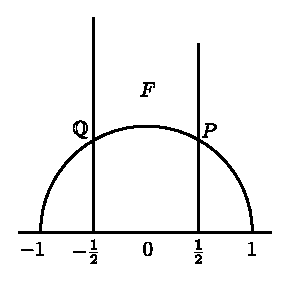
\includegraphics{fig1.eps}
\end{figure}

This\pageoriginale is the familiar modular region in the upper half
$\tau$-plane. That it is a fundamental region follows from the
properties of the space of reduced matrices in $\mathscr{P}$. The
points $P$ and $Q$ are the complex numbers $\dfrac{\pm
  1+i\sqrt{3}}{2}$, and so for any point in $F$, $\eta\geq
\dfrac{\sqrt{3}}{2}$. This means that for a positive reduced binary
form $ax^{2}+2bxy+cy^{2}$ of determinant $\ub{d}$
$$
\frac{a}{\sqrt{d}}\leq \frac{2}{\sqrt{3}},
$$
which we had already seen in Theorem \ref{chap2:thm1}.

\section{Reduction of lattices}\label{chap2:sec7}

Let $V$ be the Euclidean space of $n$ dimensions formed by $n$-rowed
real columns
$$
\alpha=
\begin{pmatrix}
a_{1}\\
\vdots\\
a_{n}
\end{pmatrix}.
$$

Let $\alpha_{1},\ldots,\alpha_{n}$ be a basis of $V$ so that
$$
\alpha_{i}=
\begin{pmatrix}
a_{1i}\\
\vdots\\
a_{ni}
\end{pmatrix},\quad i=1,\ldots,n.
$$
Denote by $A$ the matrix $(a_{kl})$. Obviously $|A|\neq 0$.

Let $L$ be a lattice in $V$ and let $\alpha_{1},\ldots,\alpha_{n}$ be
a basis of this lattice. $L$ then consists of elements
$\alpha_{1}g_{1}+\cdots+\alpha_{n}g_{n}$ where $g_{1},\ldots,g_{n}$
are integers. We shall call $A$ the {\em matrix of the lattice.}

Conversely\pageoriginale if $A$ is any non-singular $n$-rowed matrix,
then the\break columns of $A$, as elements of $V$ are linearly independent
and therefore determine a lattice.

Let $L$ be the lattice above and let $\beta_{1},\ldots,\beta_{n}$ be
any other base of $L$ and $B$ its matrix, then
$$
B=AU
$$
where $U$ is a unimodular matrix. Also if $U$ runs through all
unimodular matrices, then $AU$ runs through all bases of $L$. We now
wish to single out among these bases one which has some distinguished
properties.

Let us introduce in $V$, the inner product $\alpha\cdot\beta$ of two
vectors $\alpha$ and $\beta$ by
$$
\alpha\cdot \beta =a_{1}b_{1}+\cdots+a_{n}b_{n}
$$
where $\alpha=\left(\begin{smallmatrix}
  a_{1}\\ \vdots\\ a_{n}\end{smallmatrix}\right)$,
$\beta=\left(\begin{smallmatrix}
  b_{1}\\ \vdots\\ b_{n}\end{smallmatrix}\right)$. The square of the
length of the vector $\alpha$ is given by
$$
\alpha^{2}=a^{2}_{1}+\cdots+a^{2}_{n}.
$$

Let $A$ be the matrix of a base $\alpha_{1},\ldots,\alpha_{n}$ of
$L$. Consider the positive matrix $S=A'A$. If $S$ is given $A$ is
determined only upto an orthogonal matrix $P$ on its left. For, if
$A'A=A'_{1}A_{1}$ then $AA^{-1}_{1}=P$ is orthogonal. But
multiplication on the left by an orthogonal matrix implies a rotation
in $V$ about the origin.

We shall call a base $B$ of $L$ {\em reduced} if $S_{1}=B'B$ is a
reduced matrix. Obviously in this case 
\begin{align*}
& 0<\beta^{2}_{1}\leq\ldots\leq \beta^{2}_{n}\\
& \beta_{k}\beta_{k+1}\geq 0,\quad k=1,\ldots,n-1.
\end{align*}\pageoriginale
From the way reduced matrices are determined we see that a reduced
base $\beta_{1},\ldots,\beta_{n}$ of $L$ may be defined to be a base
such that for every set of integers $x_{1},\ldots,x_{n}$ such that
$(x_{k},\ldots,x_{n})=1$ the vector
$$
\beta=\beta_{1}x_{1}+\cdots+\beta_{n}x_{n}
$$
satisfies
$$
\beta^{2}\geq \beta^{2}_{k}\quad (k=1,\ldots,n.)
$$
Also 
$$
\beta_{k}\cdot \beta_{k+1}\geq 0(k=1,\ldots,n+1).
$$
If follows therefore that
$$
\beta^{2}_{1}\ldots\beta^{2}_{n}\leq c_{n}|A'A|=c_{n}|A|^{2}
$$
$c_{n}$ being a constant depending only on $n$. Also abs $|A|$ is the
volume of the parallelopiped formed by the vectors
$\beta_{1},\ldots,\beta_{n}$. 

consider the case $n=2$.

We have, because of \eqref{c2:eq30}
\begin{equation*}
\beta^{2}_{1}\cdot \beta^{2}_{2}\leq \frac{4}{3}|A|^{2}\tag{72}\label{c2:eq72}
\end{equation*}

Let now $\Theta$ denote the acute angle between the vectors
$\beta_{1}$ and $\beta_{2}$. Since the area of the parallelogram
formed by $\beta_{1}$ and $\beta_{2}$ on the one hand equals abs $|A|$
and on the other $\sqrt{\beta^{2}_{1}\cdot \beta^{2}_{2}}\cdot
\sin\theta$,\pageoriginale we see that
\begin{equation*}
\sin^{2}\Theta\geq \frac{3}{4}\tag{73}\label{c2:eq73}
\end{equation*}
Since $0\leq \Theta \leq \dfrac{\pi}{2}$, it follows from \eqref{c2:eq73}
that 
$$
\frac{\pi}{3}\leq \theta\leq \frac{\pi}{2}.
$$
Hence for a two dimensional lattice we may choose a basis in such a
manner that the angle (acute) between the basis vectors is between
$60^{\circ}$ and $90^{\circ}$.


\begin{thebibliography}{99}
\bibitem{c2:key1}
  C.F.\@ Gauss  {\em Disquisitiones Arithmeticae} Ges.\@ Werke 1,
(1801).

\bibitem{c2:key2} C.\@ Hermite  {\em Oeuvres} Vol.1, Paris (1905) P.\@
94-273.

\bibitem{c2:key3} H.\@ Minkowski  {\em Geometrie der Zahlen}, Leipzig (1896).

\bibitem{c2:key4} H.\@ Minkowski  Discontinuit\"atsbereich f\"ur arithmetische
Aquivalenz.  {\em Ges.\@ Werke}, Bd.2, (1911), P.53 - 100.

\bibitem{c2:key5}  C.L.\@ Siegel  Einheiten quadratischer Formen
   {\em Abh.\@ Math.\@ Sem.\@ Hansischen Univ.} 13, (1940), P.\@
   209-239.
\end{thebibliography}
